\documentclass[twoside]{book}

% Packages required by doxygen
\usepackage{fixltx2e}
\usepackage{calc}
\usepackage{doxygen}
\usepackage[export]{adjustbox} % also loads graphicx
\usepackage{graphicx}
\usepackage[utf8]{inputenc}
\usepackage{makeidx}
\usepackage{multicol}
\usepackage{multirow}
\PassOptionsToPackage{warn}{textcomp}
\usepackage{textcomp}
\usepackage[nointegrals]{wasysym}
\usepackage[table]{xcolor}

% Font selection
\usepackage[T1]{fontenc}
\usepackage[scaled=.90]{helvet}
\usepackage{courier}
\usepackage{amssymb}
\usepackage{sectsty}
\renewcommand{\familydefault}{\sfdefault}
\allsectionsfont{%
  \fontseries{bc}\selectfont%
  \color{darkgray}%
}
\renewcommand{\DoxyLabelFont}{%
  \fontseries{bc}\selectfont%
  \color{darkgray}%
}
\newcommand{\+}{\discretionary{\mbox{\scriptsize$\hookleftarrow$}}{}{}}

% Page & text layout
\usepackage{geometry}
\geometry{%
  a4paper,%
  top=2.5cm,%
  bottom=2.5cm,%
  left=2.5cm,%
  right=2.5cm%
}
\tolerance=750
\hfuzz=15pt
\hbadness=750
\setlength{\emergencystretch}{15pt}
\setlength{\parindent}{0cm}
\setlength{\parskip}{3ex plus 2ex minus 2ex}
\makeatletter
\renewcommand{\paragraph}{%
  \@startsection{paragraph}{4}{0ex}{-1.0ex}{1.0ex}{%
    \normalfont\normalsize\bfseries\SS@parafont%
  }%
}
\renewcommand{\subparagraph}{%
  \@startsection{subparagraph}{5}{0ex}{-1.0ex}{1.0ex}{%
    \normalfont\normalsize\bfseries\SS@subparafont%
  }%
}
\makeatother

% Headers & footers
\usepackage{fancyhdr}
\pagestyle{fancyplain}
\fancyhead[LE]{\fancyplain{}{\bfseries\thepage}}
\fancyhead[CE]{\fancyplain{}{}}
\fancyhead[RE]{\fancyplain{}{\bfseries\leftmark}}
\fancyhead[LO]{\fancyplain{}{\bfseries\rightmark}}
\fancyhead[CO]{\fancyplain{}{}}
\fancyhead[RO]{\fancyplain{}{\bfseries\thepage}}
\fancyfoot[LE]{\fancyplain{}{}}
\fancyfoot[CE]{\fancyplain{}{}}
\fancyfoot[RE]{\fancyplain{}{\bfseries\scriptsize Generated by Doxygen }}
\fancyfoot[LO]{\fancyplain{}{\bfseries\scriptsize Generated by Doxygen }}
\fancyfoot[CO]{\fancyplain{}{}}
\fancyfoot[RO]{\fancyplain{}{}}
\renewcommand{\footrulewidth}{0.4pt}
\renewcommand{\chaptermark}[1]{%
  \markboth{#1}{}%
}
\renewcommand{\sectionmark}[1]{%
  \markright{\thesection\ #1}%
}

% Indices & bibliography
\usepackage{natbib}
\usepackage[titles]{tocloft}
\setcounter{tocdepth}{3}
\setcounter{secnumdepth}{5}
\makeindex

% Hyperlinks (required, but should be loaded last)
\usepackage{ifpdf}
\ifpdf
  \usepackage[pdftex,pagebackref=true]{hyperref}
\else
  \usepackage[ps2pdf,pagebackref=true]{hyperref}
\fi
\hypersetup{%
  colorlinks=true,%
  linkcolor=blue,%
  citecolor=blue,%
  unicode%
}

% Custom commands
\newcommand{\clearemptydoublepage}{%
  \newpage{\pagestyle{empty}\cleardoublepage}%
}

\usepackage{caption}
\captionsetup{labelsep=space,justification=centering,font={bf},singlelinecheck=off,skip=4pt,position=top}

%===== C O N T E N T S =====

\begin{document}

% Titlepage & ToC
\hypersetup{pageanchor=false,
             bookmarksnumbered=true,
             pdfencoding=unicode
            }
\pagenumbering{roman}
\begin{titlepage}
\vspace*{7cm}
\begin{center}%
{\Large World Robot\+Interface \\[1ex]\large 1.\+0 }\\
\vspace*{1cm}
{\large Generated by Doxygen 1.8.11}\\
\end{center}
\end{titlepage}
\clearemptydoublepage
\tableofcontents
\clearemptydoublepage
\pagenumbering{arabic}
\hypersetup{pageanchor=true}

%--- Begin generated contents ---
\chapter{Namespace Index}
\section{Namespace List}
Here is a list of all documented namespaces with brief descriptions\+:\begin{DoxyCompactList}
\item\contentsline{section}{\hyperlink{namespaceMotionPlanner}{Motion\+Planner} }{\pageref{namespaceMotionPlanner}}{}
\item\contentsline{section}{\hyperlink{namespaceRobotInterface}{Robot\+Interface} }{\pageref{namespaceRobotInterface}}{}
\item\contentsline{section}{\hyperlink{namespaceRobotInterface_1_1HighLevel}{Robot\+Interface\+::\+High\+Level} }{\pageref{namespaceRobotInterface_1_1HighLevel}}{}
\item\contentsline{section}{\hyperlink{namespaceRobotInterface_1_1LowLevel}{Robot\+Interface\+::\+Low\+Level} }{\pageref{namespaceRobotInterface_1_1LowLevel}}{}
\end{DoxyCompactList}

\chapter{Hierarchical Index}
\section{Class Hierarchy}
This inheritance list is sorted roughly, but not completely, alphabetically\+:\begin{DoxyCompactList}
\item \contentsline{section}{Robot\+Interface\+:\+:High\+Level\+:\+:Command}{\pageref{classRobotInterface_1_1HighLevel_1_1Command}}{}
\item \contentsline{section}{Motion\+Planner\+:\+:Goal\+Queue\+Handler}{\pageref{classMotionPlanner_1_1GoalQueueHandler}}{}
\item \contentsline{section}{Robot\+Interface\+:\+:Low\+Level\+:\+:I\+Communication}{\pageref{classRobotInterface_1_1LowLevel_1_1ICommunication}}{}
\begin{DoxyCompactList}
\item \contentsline{section}{Robot\+Interface\+:\+:Low\+Level\+:\+:Serial\+Communication}{\pageref{classRobotInterface_1_1LowLevel_1_1SerialCommunication}}{}
\end{DoxyCompactList}
\item \contentsline{section}{Robot\+Interface\+:\+:High\+Level\+:\+:Position}{\pageref{structRobotInterface_1_1HighLevel_1_1Position}}{}
\item \contentsline{section}{Robot\+Interface\+:\+:High\+Level\+:\+:Position\+Action}{\pageref{classRobotInterface_1_1HighLevel_1_1PositionAction}}{}
\item \contentsline{section}{Motion\+Planner\+:\+:raw\+Goal}{\pageref{structMotionPlanner_1_1rawGoal}}{}
\item \contentsline{section}{Motion\+Planner\+:\+:Robot\+Interface}{\pageref{classMotionPlanner_1_1RobotInterface}}{}
\item \contentsline{section}{Robot\+Interface\+:\+:High\+Level\+:\+:Servo}{\pageref{classRobotInterface_1_1HighLevel_1_1Servo}}{}
\end{DoxyCompactList}

\chapter{Class Index}
\section{Class List}
Here are the classes, structs, unions and interfaces with brief descriptions\+:\begin{DoxyCompactList}
\item\contentsline{section}{\hyperlink{classRobotInterface_1_1HighLevel_1_1Command}{Robot\+Interface\+::\+High\+Level\+::\+Command} \\*Class that contains all information about a goal }{\pageref{classRobotInterface_1_1HighLevel_1_1Command}}{}
\item\contentsline{section}{\hyperlink{classMotionPlanner_1_1GoalQueueHandler}{Motion\+Planner\+::\+Goal\+Queue\+Handler} \\*Class that handles the queue on the server side }{\pageref{classMotionPlanner_1_1GoalQueueHandler}}{}
\item\contentsline{section}{\hyperlink{classRobotInterface_1_1LowLevel_1_1ICommunication}{Robot\+Interface\+::\+Low\+Level\+::\+I\+Communication} \\*Class that contains the lowlevel functionality. Functions that map the servo controller\textquotesingle{}s functionality For each new communication method\+: create a deriving class and override the send command function }{\pageref{classRobotInterface_1_1LowLevel_1_1ICommunication}}{}
\item\contentsline{section}{\hyperlink{structRobotInterface_1_1HighLevel_1_1Position}{Robot\+Interface\+::\+High\+Level\+::\+Position} \\*A position has a name and a map with servo indexes and positions }{\pageref{structRobotInterface_1_1HighLevel_1_1Position}}{}
\item\contentsline{section}{\hyperlink{classRobotInterface_1_1HighLevel_1_1PositionAction}{Robot\+Interface\+::\+High\+Level\+::\+Position\+Action} \\*Interface \textquotesingle{}main\textquotesingle{} (R\+O\+S-\/\+Server) }{\pageref{classRobotInterface_1_1HighLevel_1_1PositionAction}}{}
\item\contentsline{section}{\hyperlink{structMotionPlanner_1_1rawGoal}{Motion\+Planner\+::raw\+Goal} \\*Struct that contains raw goals (can easily be queued) }{\pageref{structMotionPlanner_1_1rawGoal}}{}
\item\contentsline{section}{\hyperlink{classMotionPlanner_1_1RobotInterface}{Motion\+Planner\+::\+Robot\+Interface} \\*Class that contains the demonstration and acts as \hyperlink{namespaceMotionPlanner}{Motion\+Planner} }{\pageref{classMotionPlanner_1_1RobotInterface}}{}
\item\contentsline{section}{\hyperlink{classRobotInterface_1_1LowLevel_1_1SerialCommunication}{Robot\+Interface\+::\+Low\+Level\+::\+Serial\+Communication} \\*Deriving from \hyperlink{classRobotInterface_1_1LowLevel_1_1ICommunication}{I\+Communication}\+: class that implement the send command for a serial connection }{\pageref{classRobotInterface_1_1LowLevel_1_1SerialCommunication}}{}
\item\contentsline{section}{\hyperlink{classRobotInterface_1_1HighLevel_1_1Servo}{Robot\+Interface\+::\+High\+Level\+::\+Servo} \\*This class is used for angle calculation and \hyperlink{classRobotInterface_1_1HighLevel_1_1Servo}{Servo} operations }{\pageref{classRobotInterface_1_1HighLevel_1_1Servo}}{}
\end{DoxyCompactList}

\chapter{Namespace Documentation}
\hypertarget{namespaceMotionPlanner}{}\section{Motion\+Planner Namespace Reference}
\label{namespaceMotionPlanner}\index{Motion\+Planner@{Motion\+Planner}}
\subsection*{Classes}
\begin{DoxyCompactItemize}
\item 
class \hyperlink{classMotionPlanner_1_1GoalQueueHandler}{Goal\+Queue\+Handler}
\begin{DoxyCompactList}\small\item\em Class that handles the queue on the server side. \end{DoxyCompactList}\item 
struct \hyperlink{structMotionPlanner_1_1rawGoal}{raw\+Goal}
\begin{DoxyCompactList}\small\item\em struct that contains raw goals (can easily be queued) \end{DoxyCompactList}\item 
class \hyperlink{classMotionPlanner_1_1RobotInterface}{Robot\+Interface}
\begin{DoxyCompactList}\small\item\em Class that contains the demonstration and acts as \hyperlink{namespaceMotionPlanner}{Motion\+Planner}. \end{DoxyCompactList}\end{DoxyCompactItemize}
\subsection*{Functions}
\begin{DoxyCompactItemize}
\item 
bool {\bfseries is\+Number} (const std\+::string \&s)\hypertarget{namespaceMotionPlanner_ad668551c61a3d2b30ec1e91b66be5fcc}{}\label{namespaceMotionPlanner_ad668551c61a3d2b30ec1e91b66be5fcc}

\end{DoxyCompactItemize}
\subsection*{Variables}
\begin{DoxyCompactItemize}
\item 
const unsigned short {\bfseries N\+R\+O\+F\+D\+E\+M\+O\+P\+A\+R\+A\+M\+E\+T\+E\+RS} = 2\hypertarget{namespaceMotionPlanner_afcb37e6cef602a6acc56cd8f5b085ecb}{}\label{namespaceMotionPlanner_afcb37e6cef602a6acc56cd8f5b085ecb}

\item 
const unsigned short {\bfseries N\+R\+O\+F\+P\+R\+E\+P\+R\+P\+A\+R\+A\+M\+E\+T\+E\+RS} = 3\hypertarget{namespaceMotionPlanner_acf8f40a4fe59f02df7fd5c3fac64e0b3}{}\label{namespaceMotionPlanner_acf8f40a4fe59f02df7fd5c3fac64e0b3}

\item 
const unsigned short {\bfseries M\+I\+N\+N\+R\+O\+F\+C\+U\+S\+T\+O\+M\+P\+A\+R\+A\+M\+E\+T\+E\+RS} = 4\hypertarget{namespaceMotionPlanner_a7803747ba4bcc806bf0373587a24ae9f}{}\label{namespaceMotionPlanner_a7803747ba4bcc806bf0373587a24ae9f}

\end{DoxyCompactItemize}


\subsection{Detailed Description}
The motionplanner interface contains test code that uses functionality of the \hyperlink{classMotionPlanner_1_1RobotInterface}{Robot\+Interface}. 
\hypertarget{namespaceRobotInterface}{}\section{Robot\+Interface Namespace Reference}
\label{namespaceRobotInterface}\index{Robot\+Interface@{Robot\+Interface}}
\subsection*{Namespaces}
\begin{DoxyCompactItemize}
\item 
 \hyperlink{namespaceRobotInterface_1_1HighLevel}{High\+Level}
\item 
 \hyperlink{namespaceRobotInterface_1_1LowLevel}{Low\+Level}
\end{DoxyCompactItemize}


\subsection{Detailed Description}
The interface contains a high and low -\/level driver. 
\hypertarget{namespaceRobotInterface_1_1HighLevel}{}\section{Robot\+Interface\+:\+:High\+Level Namespace Reference}
\label{namespaceRobotInterface_1_1HighLevel}\index{Robot\+Interface\+::\+High\+Level@{Robot\+Interface\+::\+High\+Level}}
\subsection*{Classes}
\begin{DoxyCompactItemize}
\item 
class \hyperlink{classRobotInterface_1_1HighLevel_1_1Command}{Command}
\begin{DoxyCompactList}\small\item\em class that contains all information about a goal. \end{DoxyCompactList}\item 
struct \hyperlink{structRobotInterface_1_1HighLevel_1_1Position}{Position}
\begin{DoxyCompactList}\small\item\em A position has a name and a map with servo indexes and positions. \end{DoxyCompactList}\item 
class \hyperlink{classRobotInterface_1_1HighLevel_1_1PositionAction}{Position\+Action}
\begin{DoxyCompactList}\small\item\em the interface \textquotesingle{}main\textquotesingle{} (R\+O\+S-\/\+Server) \end{DoxyCompactList}\item 
class \hyperlink{classRobotInterface_1_1HighLevel_1_1Servo}{Servo}
\begin{DoxyCompactList}\small\item\em This class is used for angle calculation and \hyperlink{classRobotInterface_1_1HighLevel_1_1Servo}{Servo} operations. \end{DoxyCompactList}\end{DoxyCompactItemize}
\subsection*{Enumerations}
\begin{DoxyCompactItemize}
\item 
enum \hyperlink{namespaceRobotInterface_1_1HighLevel_ab7122caf9a0b72cf97d406d33db38a7c}{States} \+: uint8\+\_\+t \{ \\*
{\bfseries C\+O\+N\+F\+I\+G\+U\+R\+A\+T\+I\+O\+N\+C\+H\+E\+CK}, 
{\bfseries I\+N\+IT}, 
{\bfseries M\+O\+V\+I\+NG}, 
{\bfseries W\+A\+I\+T\+I\+NG}, 
\\*
{\bfseries S\+T\+OP}, 
{\bfseries R\+E\+A\+D\+I\+NG}, 
{\bfseries W\+R\+I\+T\+I\+NG}
 \}
\end{DoxyCompactItemize}
\subsection*{Functions}
\begin{DoxyCompactItemize}
\item 
std\+::string {\bfseries state\+To\+Str} (const \hyperlink{namespaceRobotInterface_1_1HighLevel_ab7122caf9a0b72cf97d406d33db38a7c}{States} \&a\+State)\hypertarget{namespaceRobotInterface_1_1HighLevel_a594b969ea7a799d997d037837e7971ea}{}\label{namespaceRobotInterface_1_1HighLevel_a594b969ea7a799d997d037837e7971ea}

\end{DoxyCompactItemize}
\subsection*{Variables}
\begin{DoxyCompactItemize}
\item 
const std\+::unordered\+\_\+map$<$ std\+::string, \hyperlink{namespaceRobotInterface_1_1HighLevel_ab7122caf9a0b72cf97d406d33db38a7c}{States} $>$ \hyperlink{namespaceRobotInterface_1_1HighLevel_ac36b1d73c7eca7c1227680406f99c9b2}{states\+Map}
\end{DoxyCompactItemize}


\subsection{Detailed Description}
\hyperlink{namespaceRobotInterface_1_1HighLevel}{High\+Level} driver that contains all the high-\/level functionality of the interface. 

\subsection{Enumeration Type Documentation}
\index{Robot\+Interface\+::\+High\+Level@{Robot\+Interface\+::\+High\+Level}!States@{States}}
\index{States@{States}!Robot\+Interface\+::\+High\+Level@{Robot\+Interface\+::\+High\+Level}}
\subsubsection[{\texorpdfstring{States}{States}}]{\setlength{\rightskip}{0pt plus 5cm}enum {\bf Robot\+Interface\+::\+High\+Level\+::\+States} \+: uint8\+\_\+t\hspace{0.3cm}{\ttfamily [strong]}}\hypertarget{namespaceRobotInterface_1_1HighLevel_ab7122caf9a0b72cf97d406d33db38a7c}{}\label{namespaceRobotInterface_1_1HighLevel_ab7122caf9a0b72cf97d406d33db38a7c}
Enum that contains all the states the program can be in 

\subsection{Variable Documentation}
\index{Robot\+Interface\+::\+High\+Level@{Robot\+Interface\+::\+High\+Level}!states\+Map@{states\+Map}}
\index{states\+Map@{states\+Map}!Robot\+Interface\+::\+High\+Level@{Robot\+Interface\+::\+High\+Level}}
\subsubsection[{\texorpdfstring{states\+Map}{statesMap}}]{\setlength{\rightskip}{0pt plus 5cm}const std\+::unordered\+\_\+map$<$std\+::string, {\bf States}$>$ Robot\+Interface\+::\+High\+Level\+::states\+Map}\hypertarget{namespaceRobotInterface_1_1HighLevel_ac36b1d73c7eca7c1227680406f99c9b2}{}\label{namespaceRobotInterface_1_1HighLevel_ac36b1d73c7eca7c1227680406f99c9b2}
{\bfseries Initial value\+:}
\begin{DoxyCode}
=
    \{
        \{\textcolor{stringliteral}{"CONFIGURATIONCHECK"}, States::CONFIGURATIONCHECK\},
        \{\textcolor{stringliteral}{"INIT"}, States::INIT\},
        \{\textcolor{stringliteral}{"MOVING"}, States::MOVING\},
        \{\textcolor{stringliteral}{"WAITING"}, States::WAITING\},
        \{\textcolor{stringliteral}{"STOP"}, States::STOP\},
        \{\textcolor{stringliteral}{"READING"}, States::READING\},
        \{\textcolor{stringliteral}{"WRITING"}, States::WRITING\}\}
\end{DoxyCode}
Mapping between the states and its string representation (used for R\+OS I\+N\+FO output) 
\hypertarget{namespaceRobotInterface_1_1LowLevel}{}\section{Robot\+Interface\+:\+:Low\+Level Namespace Reference}
\label{namespaceRobotInterface_1_1LowLevel}\index{Robot\+Interface\+::\+Low\+Level@{Robot\+Interface\+::\+Low\+Level}}
\subsection*{Classes}
\begin{DoxyCompactItemize}
\item 
class \hyperlink{classRobotInterface_1_1LowLevel_1_1ICommunication}{I\+Communication}
\begin{DoxyCompactList}\small\item\em class that contains the lowlevel functionality. Functions that map the servo controller\textquotesingle{}s functionality For each new communication method\+: create a deriving class and override the send command function \end{DoxyCompactList}\item 
class \hyperlink{classRobotInterface_1_1LowLevel_1_1SerialCommunication}{Serial\+Communication}
\begin{DoxyCompactList}\small\item\em deriving from \hyperlink{classRobotInterface_1_1LowLevel_1_1ICommunication}{I\+Communication}\+: class that implement the send command for a serial connection \end{DoxyCompactList}\end{DoxyCompactItemize}


\subsection{Detailed Description}
\hyperlink{namespaceRobotInterface_1_1LowLevel}{Low\+Level} driver that contains a 1 on 1 mapping of the S\+C\+C-\/32U servo controller interface\+: only the functionality that is relevant for this exercise. 
\chapter{Class Documentation}
\hypertarget{classRobotInterface_1_1HighLevel_1_1Command}{}\section{Robot\+Interface\+:\+:High\+Level\+:\+:Command Class Reference}
\label{classRobotInterface_1_1HighLevel_1_1Command}\index{Robot\+Interface\+::\+High\+Level\+::\+Command@{Robot\+Interface\+::\+High\+Level\+::\+Command}}


class that contains all information about a goal.  




{\ttfamily \#include $<$Command.\+hpp$>$}

\subsection*{Public Member Functions}
\begin{DoxyCompactItemize}
\item 
\hyperlink{classRobotInterface_1_1HighLevel_1_1Command_ae36f803e269aa800416e1b13b27b3aa2}{Command} ()\hypertarget{classRobotInterface_1_1HighLevel_1_1Command_ae36f803e269aa800416e1b13b27b3aa2}{}\label{classRobotInterface_1_1HighLevel_1_1Command_ae36f803e269aa800416e1b13b27b3aa2}

\begin{DoxyCompactList}\small\item\em default constructor \end{DoxyCompactList}\item 
\hyperlink{classRobotInterface_1_1HighLevel_1_1Command_a08cdb5dc6b6e92be81905bc7b670f5b2}{$\sim$\+Command} ()\hypertarget{classRobotInterface_1_1HighLevel_1_1Command_a08cdb5dc6b6e92be81905bc7b670f5b2}{}\label{classRobotInterface_1_1HighLevel_1_1Command_a08cdb5dc6b6e92be81905bc7b670f5b2}

\begin{DoxyCompactList}\small\item\em destructor \end{DoxyCompactList}\item 
bool \hyperlink{classRobotInterface_1_1HighLevel_1_1Command_a2a6e0ca99d15c43627744a219b433a69}{try\+Pre\+Set\+Position} (const std\+::string \&a\+Name, unsigned long a\+Max\+Time, const std\+::vector$<$ \hyperlink{structRobotInterface_1_1HighLevel_1_1Position}{Position} $>$ \&pre\+Programmed\+Positions)
\begin{DoxyCompactList}\small\item\em function that tries to set the position of the robotic arm, based on a pre-\/programmed command (a command that is stored in the configuration file) \end{DoxyCompactList}\item 
bool \hyperlink{classRobotInterface_1_1HighLevel_1_1Command_a83f8ceeea1d0ba165574b9a70ca43594}{try\+Custom\+Position} (const std\+::map$<$ unsigned long, short $>$ \&an\+Index\+And\+Position, unsigned long a\+Max\+Time)
\begin{DoxyCompactList}\small\item\em function that tries to set the position of the robotic arm, based on arguments given on start-\/up \end{DoxyCompactList}\item 
void \hyperlink{classRobotInterface_1_1HighLevel_1_1Command_a068858e0228462ad2e793027c11aa0f5}{set\+Position} (const \hyperlink{structRobotInterface_1_1HighLevel_1_1Position}{Position} \&a\+Position)
\begin{DoxyCompactList}\small\item\em function that sets the position of a command \end{DoxyCompactList}\item 
\hyperlink{structRobotInterface_1_1HighLevel_1_1Position}{Position} \hyperlink{classRobotInterface_1_1HighLevel_1_1Command_aeca878edba659883c183686221b5ae63}{get\+Position} () const 
\begin{DoxyCompactList}\small\item\em function that returns \end{DoxyCompactList}\item 
void \hyperlink{classRobotInterface_1_1HighLevel_1_1Command_ae6cc6ca95900cefafb25285de378c0ae}{set\+Index\+And\+Position} (const std\+::map$<$ unsigned long, short $>$ \&an\+Index\+And\+Position)
\begin{DoxyCompactList}\small\item\em function that sets a mapping between servo ID\textquotesingle{}s and matching positions \end{DoxyCompactList}\item 
unsigned long \hyperlink{classRobotInterface_1_1HighLevel_1_1Command_aa4379f7948d970982971a780a928b1dc}{get\+Max\+Time} () const 
\begin{DoxyCompactList}\small\item\em getter for the maximum time a command may take \end{DoxyCompactList}\item 
bool \hyperlink{classRobotInterface_1_1HighLevel_1_1Command_ab42a68a2e06de9284b4c5b3ace882944}{validate\+Command} (const std\+::vector$<$ \hyperlink{classRobotInterface_1_1HighLevel_1_1Servo}{Servo} $>$ \&servos) const 
\begin{DoxyCompactList}\small\item\em function that validates if a command is valid or not \end{DoxyCompactList}\item 
void \hyperlink{classRobotInterface_1_1HighLevel_1_1Command_a232461097b931e8a6da3f6fab7239966}{set\+Max\+Time} (unsigned long a\+Max\+Time)
\begin{DoxyCompactList}\small\item\em setter for the maximum time the command may take \end{DoxyCompactList}\item 
void \hyperlink{classRobotInterface_1_1HighLevel_1_1Command_a7d4affca585c500be531f71794a94dc2}{set\+Emergency\+Stop} (bool an\+Emergency\+Stop)
\begin{DoxyCompactList}\small\item\em function that sets a command to be an emergency stop -\/command \end{DoxyCompactList}\item 
bool \hyperlink{classRobotInterface_1_1HighLevel_1_1Command_a02db6fe5f69006176486b1571b16dd51}{is\+Emergency\+Stop} () const 
\begin{DoxyCompactList}\small\item\em function that tells wheter the command is an emergency stop or a normal command \end{DoxyCompactList}\item 
void \hyperlink{classRobotInterface_1_1HighLevel_1_1Command_a5e7204c42507aa8c2f909703f0a7ef2e}{convert\+To\+P\+WM} (const std\+::vector$<$ \hyperlink{classRobotInterface_1_1HighLevel_1_1Servo}{Servo} $>$ \&servos)
\begin{DoxyCompactList}\small\item\em function that converts the angles set from degrees to P\+WM \end{DoxyCompactList}\item 
bool \hyperlink{classRobotInterface_1_1HighLevel_1_1Command_a5b01d427e8d2c35b07c26c03a7e8171d}{are\+Angles\+Are\+Converted} () const 
\begin{DoxyCompactList}\small\item\em function that tells if the angles are converted to P\+WM or not \end{DoxyCompactList}\item 
unsigned long \hyperlink{classRobotInterface_1_1HighLevel_1_1Command_a2f3197f1ff568af0fc757ba8d6739847}{verify\+End\+Time} () const 
\begin{DoxyCompactList}\small\item\em I\+N\+F03 requirement function that calculates wheter the robot will reach the goal in the given time and give a warning if this is not the case. \end{DoxyCompactList}\end{DoxyCompactItemize}


\subsection{Detailed Description}
class that contains all information about a goal. 

\subsection{Member Function Documentation}
\index{Robot\+Interface\+::\+High\+Level\+::\+Command@{Robot\+Interface\+::\+High\+Level\+::\+Command}!are\+Angles\+Are\+Converted@{are\+Angles\+Are\+Converted}}
\index{are\+Angles\+Are\+Converted@{are\+Angles\+Are\+Converted}!Robot\+Interface\+::\+High\+Level\+::\+Command@{Robot\+Interface\+::\+High\+Level\+::\+Command}}
\subsubsection[{\texorpdfstring{are\+Angles\+Are\+Converted() const }{areAnglesAreConverted() const }}]{\setlength{\rightskip}{0pt plus 5cm}bool Robot\+Interface\+::\+High\+Level\+::\+Command\+::are\+Angles\+Are\+Converted (
\begin{DoxyParamCaption}
{}
\end{DoxyParamCaption}
) const}\hypertarget{classRobotInterface_1_1HighLevel_1_1Command_a5b01d427e8d2c35b07c26c03a7e8171d}{}\label{classRobotInterface_1_1HighLevel_1_1Command_a5b01d427e8d2c35b07c26c03a7e8171d}


function that tells if the angles are converted to P\+WM or not 

\begin{DoxyReturn}{Returns}
true if the angles are converted to P\+WM 

false if the angles are still in degrees 
\end{DoxyReturn}
\index{Robot\+Interface\+::\+High\+Level\+::\+Command@{Robot\+Interface\+::\+High\+Level\+::\+Command}!convert\+To\+P\+WM@{convert\+To\+P\+WM}}
\index{convert\+To\+P\+WM@{convert\+To\+P\+WM}!Robot\+Interface\+::\+High\+Level\+::\+Command@{Robot\+Interface\+::\+High\+Level\+::\+Command}}
\subsubsection[{\texorpdfstring{convert\+To\+P\+W\+M(const std\+::vector$<$ Servo $>$ \&servos)}{convertToPWM(const std::vector< Servo > &servos)}}]{\setlength{\rightskip}{0pt plus 5cm}void Robot\+Interface\+::\+High\+Level\+::\+Command\+::convert\+To\+P\+WM (
\begin{DoxyParamCaption}
\item[{const std\+::vector$<$ {\bf Servo} $>$ \&}]{servos}
\end{DoxyParamCaption}
)}\hypertarget{classRobotInterface_1_1HighLevel_1_1Command_a5e7204c42507aa8c2f909703f0a7ef2e}{}\label{classRobotInterface_1_1HighLevel_1_1Command_a5e7204c42507aa8c2f909703f0a7ef2e}


function that converts the angles set from degrees to P\+WM 


\begin{DoxyParams}{Parameters}
{\em servos} & the servos that contain the information to convert an angle from degrees to P\+WM \\
\hline
\end{DoxyParams}
\index{Robot\+Interface\+::\+High\+Level\+::\+Command@{Robot\+Interface\+::\+High\+Level\+::\+Command}!get\+Max\+Time@{get\+Max\+Time}}
\index{get\+Max\+Time@{get\+Max\+Time}!Robot\+Interface\+::\+High\+Level\+::\+Command@{Robot\+Interface\+::\+High\+Level\+::\+Command}}
\subsubsection[{\texorpdfstring{get\+Max\+Time() const }{getMaxTime() const }}]{\setlength{\rightskip}{0pt plus 5cm}unsigned long Robot\+Interface\+::\+High\+Level\+::\+Command\+::get\+Max\+Time (
\begin{DoxyParamCaption}
{}
\end{DoxyParamCaption}
) const}\hypertarget{classRobotInterface_1_1HighLevel_1_1Command_aa4379f7948d970982971a780a928b1dc}{}\label{classRobotInterface_1_1HighLevel_1_1Command_aa4379f7948d970982971a780a928b1dc}


getter for the maximum time a command may take 

\begin{DoxyReturn}{Returns}
unsigned long the maximum time set 
\end{DoxyReturn}
\index{Robot\+Interface\+::\+High\+Level\+::\+Command@{Robot\+Interface\+::\+High\+Level\+::\+Command}!get\+Position@{get\+Position}}
\index{get\+Position@{get\+Position}!Robot\+Interface\+::\+High\+Level\+::\+Command@{Robot\+Interface\+::\+High\+Level\+::\+Command}}
\subsubsection[{\texorpdfstring{get\+Position() const }{getPosition() const }}]{\setlength{\rightskip}{0pt plus 5cm}{\bf Position} Robot\+Interface\+::\+High\+Level\+::\+Command\+::get\+Position (
\begin{DoxyParamCaption}
{}
\end{DoxyParamCaption}
) const}\hypertarget{classRobotInterface_1_1HighLevel_1_1Command_aeca878edba659883c183686221b5ae63}{}\label{classRobotInterface_1_1HighLevel_1_1Command_aeca878edba659883c183686221b5ae63}


function that returns 

\begin{DoxyReturn}{Returns}
\hyperlink{structRobotInterface_1_1HighLevel_1_1Position}{Position} 
\end{DoxyReturn}
\index{Robot\+Interface\+::\+High\+Level\+::\+Command@{Robot\+Interface\+::\+High\+Level\+::\+Command}!is\+Emergency\+Stop@{is\+Emergency\+Stop}}
\index{is\+Emergency\+Stop@{is\+Emergency\+Stop}!Robot\+Interface\+::\+High\+Level\+::\+Command@{Robot\+Interface\+::\+High\+Level\+::\+Command}}
\subsubsection[{\texorpdfstring{is\+Emergency\+Stop() const }{isEmergencyStop() const }}]{\setlength{\rightskip}{0pt plus 5cm}bool Robot\+Interface\+::\+High\+Level\+::\+Command\+::is\+Emergency\+Stop (
\begin{DoxyParamCaption}
{}
\end{DoxyParamCaption}
) const}\hypertarget{classRobotInterface_1_1HighLevel_1_1Command_a02db6fe5f69006176486b1571b16dd51}{}\label{classRobotInterface_1_1HighLevel_1_1Command_a02db6fe5f69006176486b1571b16dd51}


function that tells wheter the command is an emergency stop or a normal command 

\begin{DoxyReturn}{Returns}
true if the command is an emergency stop 

false if the command is a normal command 
\end{DoxyReturn}
\index{Robot\+Interface\+::\+High\+Level\+::\+Command@{Robot\+Interface\+::\+High\+Level\+::\+Command}!set\+Emergency\+Stop@{set\+Emergency\+Stop}}
\index{set\+Emergency\+Stop@{set\+Emergency\+Stop}!Robot\+Interface\+::\+High\+Level\+::\+Command@{Robot\+Interface\+::\+High\+Level\+::\+Command}}
\subsubsection[{\texorpdfstring{set\+Emergency\+Stop(bool an\+Emergency\+Stop)}{setEmergencyStop(bool anEmergencyStop)}}]{\setlength{\rightskip}{0pt plus 5cm}void Robot\+Interface\+::\+High\+Level\+::\+Command\+::set\+Emergency\+Stop (
\begin{DoxyParamCaption}
\item[{bool}]{an\+Emergency\+Stop}
\end{DoxyParamCaption}
)}\hypertarget{classRobotInterface_1_1HighLevel_1_1Command_a7d4affca585c500be531f71794a94dc2}{}\label{classRobotInterface_1_1HighLevel_1_1Command_a7d4affca585c500be531f71794a94dc2}


function that sets a command to be an emergency stop -\/command 


\begin{DoxyParams}{Parameters}
{\em an\+Emergency\+Stop} & true for an emergency stop, false if not \\
\hline
\end{DoxyParams}
\index{Robot\+Interface\+::\+High\+Level\+::\+Command@{Robot\+Interface\+::\+High\+Level\+::\+Command}!set\+Index\+And\+Position@{set\+Index\+And\+Position}}
\index{set\+Index\+And\+Position@{set\+Index\+And\+Position}!Robot\+Interface\+::\+High\+Level\+::\+Command@{Robot\+Interface\+::\+High\+Level\+::\+Command}}
\subsubsection[{\texorpdfstring{set\+Index\+And\+Position(const std\+::map$<$ unsigned long, short $>$ \&an\+Index\+And\+Position)}{setIndexAndPosition(const std::map< unsigned long, short > &anIndexAndPosition)}}]{\setlength{\rightskip}{0pt plus 5cm}void Robot\+Interface\+::\+High\+Level\+::\+Command\+::set\+Index\+And\+Position (
\begin{DoxyParamCaption}
\item[{const std\+::map$<$ unsigned long, short $>$ \&}]{an\+Index\+And\+Position}
\end{DoxyParamCaption}
)}\hypertarget{classRobotInterface_1_1HighLevel_1_1Command_ae6cc6ca95900cefafb25285de378c0ae}{}\label{classRobotInterface_1_1HighLevel_1_1Command_ae6cc6ca95900cefafb25285de378c0ae}


function that sets a mapping between servo ID\textquotesingle{}s and matching positions 


\begin{DoxyParams}{Parameters}
{\em an\+Index\+And\+Position} & \\
\hline
\end{DoxyParams}
\index{Robot\+Interface\+::\+High\+Level\+::\+Command@{Robot\+Interface\+::\+High\+Level\+::\+Command}!set\+Max\+Time@{set\+Max\+Time}}
\index{set\+Max\+Time@{set\+Max\+Time}!Robot\+Interface\+::\+High\+Level\+::\+Command@{Robot\+Interface\+::\+High\+Level\+::\+Command}}
\subsubsection[{\texorpdfstring{set\+Max\+Time(unsigned long a\+Max\+Time)}{setMaxTime(unsigned long aMaxTime)}}]{\setlength{\rightskip}{0pt plus 5cm}void Robot\+Interface\+::\+High\+Level\+::\+Command\+::set\+Max\+Time (
\begin{DoxyParamCaption}
\item[{unsigned long}]{a\+Max\+Time}
\end{DoxyParamCaption}
)}\hypertarget{classRobotInterface_1_1HighLevel_1_1Command_a232461097b931e8a6da3f6fab7239966}{}\label{classRobotInterface_1_1HighLevel_1_1Command_a232461097b931e8a6da3f6fab7239966}


setter for the maximum time the command may take 


\begin{DoxyParams}{Parameters}
{\em a\+Max\+Time} & the maximum time a command may take \\
\hline
\end{DoxyParams}
\index{Robot\+Interface\+::\+High\+Level\+::\+Command@{Robot\+Interface\+::\+High\+Level\+::\+Command}!set\+Position@{set\+Position}}
\index{set\+Position@{set\+Position}!Robot\+Interface\+::\+High\+Level\+::\+Command@{Robot\+Interface\+::\+High\+Level\+::\+Command}}
\subsubsection[{\texorpdfstring{set\+Position(const Position \&a\+Position)}{setPosition(const Position &aPosition)}}]{\setlength{\rightskip}{0pt plus 5cm}void Robot\+Interface\+::\+High\+Level\+::\+Command\+::set\+Position (
\begin{DoxyParamCaption}
\item[{const {\bf Position} \&}]{a\+Position}
\end{DoxyParamCaption}
)}\hypertarget{classRobotInterface_1_1HighLevel_1_1Command_a068858e0228462ad2e793027c11aa0f5}{}\label{classRobotInterface_1_1HighLevel_1_1Command_a068858e0228462ad2e793027c11aa0f5}


function that sets the position of a command 


\begin{DoxyParams}{Parameters}
{\em a\+Position} & the position to be set \\
\hline
\end{DoxyParams}
\index{Robot\+Interface\+::\+High\+Level\+::\+Command@{Robot\+Interface\+::\+High\+Level\+::\+Command}!try\+Custom\+Position@{try\+Custom\+Position}}
\index{try\+Custom\+Position@{try\+Custom\+Position}!Robot\+Interface\+::\+High\+Level\+::\+Command@{Robot\+Interface\+::\+High\+Level\+::\+Command}}
\subsubsection[{\texorpdfstring{try\+Custom\+Position(const std\+::map$<$ unsigned long, short $>$ \&an\+Index\+And\+Position, unsigned long a\+Max\+Time)}{tryCustomPosition(const std::map< unsigned long, short > &anIndexAndPosition, unsigned long aMaxTime)}}]{\setlength{\rightskip}{0pt plus 5cm}bool Robot\+Interface\+::\+High\+Level\+::\+Command\+::try\+Custom\+Position (
\begin{DoxyParamCaption}
\item[{const std\+::map$<$ unsigned long, short $>$ \&}]{an\+Index\+And\+Position, }
\item[{unsigned long}]{a\+Max\+Time}
\end{DoxyParamCaption}
)}\hypertarget{classRobotInterface_1_1HighLevel_1_1Command_a83f8ceeea1d0ba165574b9a70ca43594}{}\label{classRobotInterface_1_1HighLevel_1_1Command_a83f8ceeea1d0ba165574b9a70ca43594}


function that tries to set the position of the robotic arm, based on arguments given on start-\/up 


\begin{DoxyParams}{Parameters}
{\em an\+Index\+And\+Position} & a map where the ID of a specific servo is on the index side, and the position (in degrees) is on the right side \\
\hline
{\em a\+Max\+Time} & the maximum time the robotic arm is allowed to take to execute the command \\
\hline
\end{DoxyParams}
\begin{DoxyReturn}{Returns}
bool true if the command exists and can be executed, false if not 
\end{DoxyReturn}
\index{Robot\+Interface\+::\+High\+Level\+::\+Command@{Robot\+Interface\+::\+High\+Level\+::\+Command}!try\+Pre\+Set\+Position@{try\+Pre\+Set\+Position}}
\index{try\+Pre\+Set\+Position@{try\+Pre\+Set\+Position}!Robot\+Interface\+::\+High\+Level\+::\+Command@{Robot\+Interface\+::\+High\+Level\+::\+Command}}
\subsubsection[{\texorpdfstring{try\+Pre\+Set\+Position(const std\+::string \&a\+Name, unsigned long a\+Max\+Time, const std\+::vector$<$ Position $>$ \&pre\+Programmed\+Positions)}{tryPreSetPosition(const std::string &aName, unsigned long aMaxTime, const std::vector< Position > &preProgrammedPositions)}}]{\setlength{\rightskip}{0pt plus 5cm}bool Robot\+Interface\+::\+High\+Level\+::\+Command\+::try\+Pre\+Set\+Position (
\begin{DoxyParamCaption}
\item[{const std\+::string \&}]{a\+Name, }
\item[{unsigned long}]{a\+Max\+Time, }
\item[{const std\+::vector$<$ {\bf Position} $>$ \&}]{pre\+Programmed\+Positions}
\end{DoxyParamCaption}
)}\hypertarget{classRobotInterface_1_1HighLevel_1_1Command_a2a6e0ca99d15c43627744a219b433a69}{}\label{classRobotInterface_1_1HighLevel_1_1Command_a2a6e0ca99d15c43627744a219b433a69}


function that tries to set the position of the robotic arm, based on a pre-\/programmed command (a command that is stored in the configuration file) 


\begin{DoxyParams}{Parameters}
{\em a\+Name} & the name of the pre-\/programmed position that is requested \\
\hline
{\em a\+Max\+Time} & the maximum time the robotic arm is allowed to take to execute the command \\
\hline
{\em pre\+Programmed\+Positions} & a reference to the list with the pre-\/programmed positions \\
\hline
\end{DoxyParams}
\begin{DoxyReturn}{Returns}
bool true if the command exists and can be executed, false if not 
\end{DoxyReturn}
\index{Robot\+Interface\+::\+High\+Level\+::\+Command@{Robot\+Interface\+::\+High\+Level\+::\+Command}!validate\+Command@{validate\+Command}}
\index{validate\+Command@{validate\+Command}!Robot\+Interface\+::\+High\+Level\+::\+Command@{Robot\+Interface\+::\+High\+Level\+::\+Command}}
\subsubsection[{\texorpdfstring{validate\+Command(const std\+::vector$<$ Servo $>$ \&servos) const }{validateCommand(const std::vector< Servo > &servos) const }}]{\setlength{\rightskip}{0pt plus 5cm}bool Robot\+Interface\+::\+High\+Level\+::\+Command\+::validate\+Command (
\begin{DoxyParamCaption}
\item[{const std\+::vector$<$ {\bf Servo} $>$ \&}]{servos}
\end{DoxyParamCaption}
) const}\hypertarget{classRobotInterface_1_1HighLevel_1_1Command_ab42a68a2e06de9284b4c5b3ace882944}{}\label{classRobotInterface_1_1HighLevel_1_1Command_ab42a68a2e06de9284b4c5b3ace882944}


function that validates if a command is valid or not 


\begin{DoxyParams}{Parameters}
{\em servos} & the servos that contain information about minimum and maximum positions a servo may be in \\
\hline
\end{DoxyParams}
\begin{DoxyReturn}{Returns}
true if a command is validated 

false if a command is not valid 
\end{DoxyReturn}
\index{Robot\+Interface\+::\+High\+Level\+::\+Command@{Robot\+Interface\+::\+High\+Level\+::\+Command}!verify\+End\+Time@{verify\+End\+Time}}
\index{verify\+End\+Time@{verify\+End\+Time}!Robot\+Interface\+::\+High\+Level\+::\+Command@{Robot\+Interface\+::\+High\+Level\+::\+Command}}
\subsubsection[{\texorpdfstring{verify\+End\+Time() const }{verifyEndTime() const }}]{\setlength{\rightskip}{0pt plus 5cm}unsigned long Robot\+Interface\+::\+High\+Level\+::\+Command\+::verify\+End\+Time (
\begin{DoxyParamCaption}
{}
\end{DoxyParamCaption}
) const}\hypertarget{classRobotInterface_1_1HighLevel_1_1Command_a2f3197f1ff568af0fc757ba8d6739847}{}\label{classRobotInterface_1_1HighLevel_1_1Command_a2f3197f1ff568af0fc757ba8d6739847}


I\+N\+F03 requirement function that calculates wheter the robot will reach the goal in the given time and give a warning if this is not the case. 

\begin{DoxyReturn}{Returns}
unsigned long the expected end time 
\end{DoxyReturn}
The slowest servo attatched to the Lynx\+Motion can move 180 d egrees in 0.\+84 seconds

Source\+: Attachments\+: \char`\"{}hs755hb.\+pdf\char`\"{} \begin{DoxyVerb}If the requested maxTime is bigger than 
\end{DoxyVerb}
 the max moving time the robot will reach the position in the requested time 

The documentation for this class was generated from the following files\+:\begin{DoxyCompactItemize}
\item 
world\+\_\+ws/src/robot\+\_\+interface/src/\+Robot\+Interface/\+High\+Level/Command.\+hpp\item 
world\+\_\+ws/src/robot\+\_\+interface/src/\+Robot\+Interface/\+High\+Level/Command.\+cpp\end{DoxyCompactItemize}

\hypertarget{classMotionPlanner_1_1GoalQueueHandler}{}\section{Motion\+Planner\+:\+:Goal\+Queue\+Handler Class Reference}
\label{classMotionPlanner_1_1GoalQueueHandler}\index{Motion\+Planner\+::\+Goal\+Queue\+Handler@{Motion\+Planner\+::\+Goal\+Queue\+Handler}}


Class that handles the queue on the server side.  




{\ttfamily \#include $<$Goal\+Queue\+Handler.\+hpp$>$}

\subsection*{Public Member Functions}
\begin{DoxyCompactItemize}
\item 
\hyperlink{classMotionPlanner_1_1GoalQueueHandler_a74cbd86f98f2f0b236213041b1e6f32b}{Goal\+Queue\+Handler} ()\hypertarget{classMotionPlanner_1_1GoalQueueHandler_a74cbd86f98f2f0b236213041b1e6f32b}{}\label{classMotionPlanner_1_1GoalQueueHandler_a74cbd86f98f2f0b236213041b1e6f32b}

\begin{DoxyCompactList}\small\item\em Construct a new Goal Queue Handler object. \end{DoxyCompactList}\item 
\hyperlink{classMotionPlanner_1_1GoalQueueHandler_a9aad546d5899b57dd4f08d5ae20125f1}{$\sim$\+Goal\+Queue\+Handler} ()\hypertarget{classMotionPlanner_1_1GoalQueueHandler_a9aad546d5899b57dd4f08d5ae20125f1}{}\label{classMotionPlanner_1_1GoalQueueHandler_a9aad546d5899b57dd4f08d5ae20125f1}

\begin{DoxyCompactList}\small\item\em Destroy the Goal Queue Handler object. \end{DoxyCompactList}\item 
void \hyperlink{classMotionPlanner_1_1GoalQueueHandler_aac7538d38c2f327c563cb0e962a18ece}{add\+Raw\+Goal} (int argc, char $\ast$argv\mbox{[}$\,$\mbox{]})
\begin{DoxyCompactList}\small\item\em function that will try to set a goal based on the commandline arguments \end{DoxyCompactList}\item 
void \hyperlink{classMotionPlanner_1_1GoalQueueHandler_a4f08a02fca360c8010f9d324784acf28}{add\+Goal} (const \hyperlink{structMotionPlanner_1_1rawGoal}{raw\+Goal} \&a\+Raw\+Goal)
\begin{DoxyCompactList}\small\item\em function that adds a goal to the queue \end{DoxyCompactList}\item 
std\+::queue$<$ \hyperlink{structMotionPlanner_1_1rawGoal}{raw\+Goal} $>$ \hyperlink{classMotionPlanner_1_1GoalQueueHandler_a6ee31f36ec20b2e9b16d14ee9af06cfe}{get\+Queue} () const 
\begin{DoxyCompactList}\small\item\em Get the Queue object. \end{DoxyCompactList}\item 
robot\+\_\+interface\+::\+Position\+Goal \hyperlink{classMotionPlanner_1_1GoalQueueHandler_a8f82872be4c475e58b061fc96b525fc6}{get\+Next\+Goal} ()
\begin{DoxyCompactList}\small\item\em Get the Next Goal object. \end{DoxyCompactList}\item 
void \hyperlink{classMotionPlanner_1_1GoalQueueHandler_a249e898b831fe6619f607f77cacdfd5d}{clear} ()\hypertarget{classMotionPlanner_1_1GoalQueueHandler_a249e898b831fe6619f607f77cacdfd5d}{}\label{classMotionPlanner_1_1GoalQueueHandler_a249e898b831fe6619f607f77cacdfd5d}

\begin{DoxyCompactList}\small\item\em Function that empties the current queue. \end{DoxyCompactList}\end{DoxyCompactItemize}


\subsection{Detailed Description}
Class that handles the queue on the server side. 

\subsection{Member Function Documentation}
\index{Motion\+Planner\+::\+Goal\+Queue\+Handler@{Motion\+Planner\+::\+Goal\+Queue\+Handler}!add\+Goal@{add\+Goal}}
\index{add\+Goal@{add\+Goal}!Motion\+Planner\+::\+Goal\+Queue\+Handler@{Motion\+Planner\+::\+Goal\+Queue\+Handler}}
\subsubsection[{\texorpdfstring{add\+Goal(const raw\+Goal \&a\+Raw\+Goal)}{addGoal(const rawGoal &aRawGoal)}}]{\setlength{\rightskip}{0pt plus 5cm}void Motion\+Planner\+::\+Goal\+Queue\+Handler\+::add\+Goal (
\begin{DoxyParamCaption}
\item[{const {\bf raw\+Goal} \&}]{a\+Raw\+Goal}
\end{DoxyParamCaption}
)}\hypertarget{classMotionPlanner_1_1GoalQueueHandler_a4f08a02fca360c8010f9d324784acf28}{}\label{classMotionPlanner_1_1GoalQueueHandler_a4f08a02fca360c8010f9d324784acf28}


function that adds a goal to the queue 


\begin{DoxyParams}{Parameters}
{\em a\+Raw\+Goal} & the goal to be added \\
\hline
\end{DoxyParams}
\index{Motion\+Planner\+::\+Goal\+Queue\+Handler@{Motion\+Planner\+::\+Goal\+Queue\+Handler}!add\+Raw\+Goal@{add\+Raw\+Goal}}
\index{add\+Raw\+Goal@{add\+Raw\+Goal}!Motion\+Planner\+::\+Goal\+Queue\+Handler@{Motion\+Planner\+::\+Goal\+Queue\+Handler}}
\subsubsection[{\texorpdfstring{add\+Raw\+Goal(int argc, char $\ast$argv[])}{addRawGoal(int argc, char *argv[])}}]{\setlength{\rightskip}{0pt plus 5cm}void Motion\+Planner\+::\+Goal\+Queue\+Handler\+::add\+Raw\+Goal (
\begin{DoxyParamCaption}
\item[{int}]{argc, }
\item[{char $\ast$}]{argv\mbox{[}$\,$\mbox{]}}
\end{DoxyParamCaption}
)}\hypertarget{classMotionPlanner_1_1GoalQueueHandler_aac7538d38c2f327c563cb0e962a18ece}{}\label{classMotionPlanner_1_1GoalQueueHandler_aac7538d38c2f327c563cb0e962a18ece}


function that will try to set a goal based on the commandline arguments 


\begin{DoxyParams}{Parameters}
{\em argc} & the number of arguments given by the user \\
\hline
{\em argv} & array with the arguments \\
\hline
\end{DoxyParams}

\begin{DoxyExceptions}{Exceptions}
{\em if} & no goal could be created based on the commandline arguments \\
\hline
\end{DoxyExceptions}
\index{Motion\+Planner\+::\+Goal\+Queue\+Handler@{Motion\+Planner\+::\+Goal\+Queue\+Handler}!get\+Next\+Goal@{get\+Next\+Goal}}
\index{get\+Next\+Goal@{get\+Next\+Goal}!Motion\+Planner\+::\+Goal\+Queue\+Handler@{Motion\+Planner\+::\+Goal\+Queue\+Handler}}
\subsubsection[{\texorpdfstring{get\+Next\+Goal()}{getNextGoal()}}]{\setlength{\rightskip}{0pt plus 5cm}robot\+\_\+interface\+::\+Position\+Goal Motion\+Planner\+::\+Goal\+Queue\+Handler\+::get\+Next\+Goal (
\begin{DoxyParamCaption}
{}
\end{DoxyParamCaption}
)}\hypertarget{classMotionPlanner_1_1GoalQueueHandler_a8f82872be4c475e58b061fc96b525fc6}{}\label{classMotionPlanner_1_1GoalQueueHandler_a8f82872be4c475e58b061fc96b525fc6}


Get the Next Goal object. 

\begin{DoxyReturn}{Returns}
robot\+\_\+interface\+::\+Position\+Goal 
\end{DoxyReturn}
\index{Motion\+Planner\+::\+Goal\+Queue\+Handler@{Motion\+Planner\+::\+Goal\+Queue\+Handler}!get\+Queue@{get\+Queue}}
\index{get\+Queue@{get\+Queue}!Motion\+Planner\+::\+Goal\+Queue\+Handler@{Motion\+Planner\+::\+Goal\+Queue\+Handler}}
\subsubsection[{\texorpdfstring{get\+Queue() const }{getQueue() const }}]{\setlength{\rightskip}{0pt plus 5cm}std\+::queue$<$ {\bf raw\+Goal} $>$ Motion\+Planner\+::\+Goal\+Queue\+Handler\+::get\+Queue (
\begin{DoxyParamCaption}
{}
\end{DoxyParamCaption}
) const}\hypertarget{classMotionPlanner_1_1GoalQueueHandler_a6ee31f36ec20b2e9b16d14ee9af06cfe}{}\label{classMotionPlanner_1_1GoalQueueHandler_a6ee31f36ec20b2e9b16d14ee9af06cfe}


Get the Queue object. 

\begin{DoxyReturn}{Returns}
std\+::queue$<$raw\+Goal$>$ 
\end{DoxyReturn}


The documentation for this class was generated from the following files\+:\begin{DoxyCompactItemize}
\item 
world\+\_\+ws/src/robot\+\_\+interface/src/\+Motion\+Planner/Goal\+Queue\+Handler.\+hpp\item 
world\+\_\+ws/src/robot\+\_\+interface/src/\+Motion\+Planner/Goal\+Queue\+Handler.\+cpp\end{DoxyCompactItemize}

\hypertarget{classRobotInterface_1_1LowLevel_1_1ICommunication}{}\section{Robot\+Interface\+:\+:Low\+Level\+:\+:I\+Communication Class Reference}
\label{classRobotInterface_1_1LowLevel_1_1ICommunication}\index{Robot\+Interface\+::\+Low\+Level\+::\+I\+Communication@{Robot\+Interface\+::\+Low\+Level\+::\+I\+Communication}}


class that contains the lowlevel functionality. Functions that map the servo controller\textquotesingle{}s functionality For each new communication method\+: create a deriving class and override the send command function  




{\ttfamily \#include $<$I\+Communication.\+hpp$>$}



Inheritance diagram for Robot\+Interface\+:\+:Low\+Level\+:\+:I\+Communication\+:
\nopagebreak
\begin{figure}[H]
\begin{center}
\leavevmode
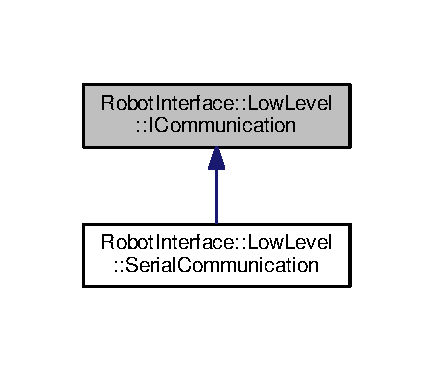
\includegraphics[width=208pt]{classRobotInterface_1_1LowLevel_1_1ICommunication__inherit__graph}
\end{center}
\end{figure}
\subsection*{Public Member Functions}
\begin{DoxyCompactItemize}
\item 
\hyperlink{classRobotInterface_1_1LowLevel_1_1ICommunication_a549d6cec59f9acc7bae341201581c71a}{I\+Communication} ()\hypertarget{classRobotInterface_1_1LowLevel_1_1ICommunication_a549d6cec59f9acc7bae341201581c71a}{}\label{classRobotInterface_1_1LowLevel_1_1ICommunication_a549d6cec59f9acc7bae341201581c71a}

\begin{DoxyCompactList}\small\item\em default constructor \end{DoxyCompactList}\item 
virtual \hyperlink{classRobotInterface_1_1LowLevel_1_1ICommunication_a74a38bd2d01f632ec2dfc88702c768d5}{$\sim$\+I\+Communication} ()\hypertarget{classRobotInterface_1_1LowLevel_1_1ICommunication_a74a38bd2d01f632ec2dfc88702c768d5}{}\label{classRobotInterface_1_1LowLevel_1_1ICommunication_a74a38bd2d01f632ec2dfc88702c768d5}

\begin{DoxyCompactList}\small\item\em destructor \end{DoxyCompactList}\item 
virtual bool \hyperlink{classRobotInterface_1_1LowLevel_1_1ICommunication_a88fc73dd43eb0444895e1a8b33fc1623}{send\+Command} (const std\+::string \&str)=0
\begin{DoxyCompactList}\small\item\em validates send goal and sends it to the S\+S\+C32U \end{DoxyCompactList}\item 
std\+::string \hyperlink{classRobotInterface_1_1LowLevel_1_1ICommunication_aece444b8550301f7d65d1580581a1e62}{position\+Speed\+Command\+To\+Str} (const std\+::map$<$ unsigned long, short $>$ \&index\+And\+Position, long speed)
\begin{DoxyCompactList}\small\item\em function that sets a position command with a speed indication to string form \end{DoxyCompactList}\item 
std\+::string \hyperlink{classRobotInterface_1_1LowLevel_1_1ICommunication_a107a620b30d9aef6565bbe26a6308b73}{emergency\+Stop\+Command\+To\+Str} (const std\+::map$<$ unsigned long, short $>$ \&index\+And\+Position)
\begin{DoxyCompactList}\small\item\em function that sends an emergency stop command to the robot \end{DoxyCompactList}\item 
std\+::string \hyperlink{classRobotInterface_1_1LowLevel_1_1ICommunication_a92c27d361d72d13460ee20c3241c4a5d}{position\+Time\+Command\+To\+Str} (const std\+::map$<$ unsigned long, short $>$ \&index\+And\+Position, long max\+Time)
\begin{DoxyCompactList}\small\item\em function that creates a string representation of a low level S\+S\+C32U command \end{DoxyCompactList}\end{DoxyCompactItemize}


\subsection{Detailed Description}
class that contains the lowlevel functionality. Functions that map the servo controller\textquotesingle{}s functionality For each new communication method\+: create a deriving class and override the send command function 

\subsection{Member Function Documentation}
\index{Robot\+Interface\+::\+Low\+Level\+::\+I\+Communication@{Robot\+Interface\+::\+Low\+Level\+::\+I\+Communication}!emergency\+Stop\+Command\+To\+Str@{emergency\+Stop\+Command\+To\+Str}}
\index{emergency\+Stop\+Command\+To\+Str@{emergency\+Stop\+Command\+To\+Str}!Robot\+Interface\+::\+Low\+Level\+::\+I\+Communication@{Robot\+Interface\+::\+Low\+Level\+::\+I\+Communication}}
\subsubsection[{\texorpdfstring{emergency\+Stop\+Command\+To\+Str(const std\+::map$<$ unsigned long, short $>$ \&index\+And\+Position)}{emergencyStopCommandToStr(const std::map< unsigned long, short > &indexAndPosition)}}]{\setlength{\rightskip}{0pt plus 5cm}std\+::string Robot\+Interface\+::\+Low\+Level\+::\+I\+Communication\+::emergency\+Stop\+Command\+To\+Str (
\begin{DoxyParamCaption}
\item[{const std\+::map$<$ unsigned long, short $>$ \&}]{index\+And\+Position}
\end{DoxyParamCaption}
)}\hypertarget{classRobotInterface_1_1LowLevel_1_1ICommunication_a107a620b30d9aef6565bbe26a6308b73}{}\label{classRobotInterface_1_1LowLevel_1_1ICommunication_a107a620b30d9aef6565bbe26a6308b73}


function that sends an emergency stop command to the robot 


\begin{DoxyParams}{Parameters}
{\em index\+And\+Position} & mapping beteween servo id\textquotesingle{}s and the position in P\+WM the servo should move to \\
\hline
\end{DoxyParams}
\begin{DoxyReturn}{Returns}
std\+::string the string representation of the command 
\end{DoxyReturn}
\index{Robot\+Interface\+::\+Low\+Level\+::\+I\+Communication@{Robot\+Interface\+::\+Low\+Level\+::\+I\+Communication}!position\+Speed\+Command\+To\+Str@{position\+Speed\+Command\+To\+Str}}
\index{position\+Speed\+Command\+To\+Str@{position\+Speed\+Command\+To\+Str}!Robot\+Interface\+::\+Low\+Level\+::\+I\+Communication@{Robot\+Interface\+::\+Low\+Level\+::\+I\+Communication}}
\subsubsection[{\texorpdfstring{position\+Speed\+Command\+To\+Str(const std\+::map$<$ unsigned long, short $>$ \&index\+And\+Position, long speed)}{positionSpeedCommandToStr(const std::map< unsigned long, short > &indexAndPosition, long speed)}}]{\setlength{\rightskip}{0pt plus 5cm}std\+::string Robot\+Interface\+::\+Low\+Level\+::\+I\+Communication\+::position\+Speed\+Command\+To\+Str (
\begin{DoxyParamCaption}
\item[{const std\+::map$<$ unsigned long, short $>$ \&}]{index\+And\+Position, }
\item[{long}]{speed}
\end{DoxyParamCaption}
)}\hypertarget{classRobotInterface_1_1LowLevel_1_1ICommunication_aece444b8550301f7d65d1580581a1e62}{}\label{classRobotInterface_1_1LowLevel_1_1ICommunication_aece444b8550301f7d65d1580581a1e62}


function that sets a position command with a speed indication to string form 


\begin{DoxyParams}{Parameters}
{\em index\+And\+Position} & mapping beteween servo id\textquotesingle{}s and the position in P\+WM the servo should move to \\
\hline
{\em speed} & the speed in US \\
\hline
\end{DoxyParams}
\begin{DoxyReturn}{Returns}
std\+::string the command converted to a string 
\end{DoxyReturn}
\index{Robot\+Interface\+::\+Low\+Level\+::\+I\+Communication@{Robot\+Interface\+::\+Low\+Level\+::\+I\+Communication}!position\+Time\+Command\+To\+Str@{position\+Time\+Command\+To\+Str}}
\index{position\+Time\+Command\+To\+Str@{position\+Time\+Command\+To\+Str}!Robot\+Interface\+::\+Low\+Level\+::\+I\+Communication@{Robot\+Interface\+::\+Low\+Level\+::\+I\+Communication}}
\subsubsection[{\texorpdfstring{position\+Time\+Command\+To\+Str(const std\+::map$<$ unsigned long, short $>$ \&index\+And\+Position, long max\+Time)}{positionTimeCommandToStr(const std::map< unsigned long, short > &indexAndPosition, long maxTime)}}]{\setlength{\rightskip}{0pt plus 5cm}std\+::string Robot\+Interface\+::\+Low\+Level\+::\+I\+Communication\+::position\+Time\+Command\+To\+Str (
\begin{DoxyParamCaption}
\item[{const std\+::map$<$ unsigned long, short $>$ \&}]{index\+And\+Position, }
\item[{long}]{max\+Time}
\end{DoxyParamCaption}
)}\hypertarget{classRobotInterface_1_1LowLevel_1_1ICommunication_a92c27d361d72d13460ee20c3241c4a5d}{}\label{classRobotInterface_1_1LowLevel_1_1ICommunication_a92c27d361d72d13460ee20c3241c4a5d}


function that creates a string representation of a low level S\+S\+C32U command 


\begin{DoxyParams}{Parameters}
{\em index\+And\+Position} & mapping beteween servo id\textquotesingle{}s and the position in P\+WM the servo should move to \\
\hline
{\em max\+Time} & the maximum time a command may take \\
\hline
\end{DoxyParams}
\begin{DoxyReturn}{Returns}
std\+::string the string representation of the low level S\+S\+C32U command 
\end{DoxyReturn}
\index{Robot\+Interface\+::\+Low\+Level\+::\+I\+Communication@{Robot\+Interface\+::\+Low\+Level\+::\+I\+Communication}!send\+Command@{send\+Command}}
\index{send\+Command@{send\+Command}!Robot\+Interface\+::\+Low\+Level\+::\+I\+Communication@{Robot\+Interface\+::\+Low\+Level\+::\+I\+Communication}}
\subsubsection[{\texorpdfstring{send\+Command(const std\+::string \&str)=0}{sendCommand(const std::string &str)=0}}]{\setlength{\rightskip}{0pt plus 5cm}virtual bool Robot\+Interface\+::\+Low\+Level\+::\+I\+Communication\+::send\+Command (
\begin{DoxyParamCaption}
\item[{const std\+::string \&}]{str}
\end{DoxyParamCaption}
)\hspace{0.3cm}{\ttfamily [pure virtual]}}\hypertarget{classRobotInterface_1_1LowLevel_1_1ICommunication_a88fc73dd43eb0444895e1a8b33fc1623}{}\label{classRobotInterface_1_1LowLevel_1_1ICommunication_a88fc73dd43eb0444895e1a8b33fc1623}


validates send goal and sends it to the S\+S\+C32U 

\begin{DoxyReturn}{Returns}
true if goal is reachable 

false if goal is unreachable 
\end{DoxyReturn}


Implemented in \hyperlink{classRobotInterface_1_1LowLevel_1_1SerialCommunication_a82fe3bcbc561e158ab7722f7182a97d7}{Robot\+Interface\+::\+Low\+Level\+::\+Serial\+Communication}.



The documentation for this class was generated from the following files\+:\begin{DoxyCompactItemize}
\item 
world\+\_\+ws/src/robot\+\_\+interface/src/\+Robot\+Interface/\+Low\+Level/I\+Communication.\+hpp\item 
world\+\_\+ws/src/robot\+\_\+interface/src/\+Robot\+Interface/\+Low\+Level/I\+Communication.\+cpp\end{DoxyCompactItemize}

\hypertarget{structRobotInterface_1_1HighLevel_1_1Position}{}\section{Robot\+Interface\+:\+:High\+Level\+:\+:Position Struct Reference}
\label{structRobotInterface_1_1HighLevel_1_1Position}\index{Robot\+Interface\+::\+High\+Level\+::\+Position@{Robot\+Interface\+::\+High\+Level\+::\+Position}}


A position has a name and a map with servo indexes and positions.  




{\ttfamily \#include $<$Position.\+hpp$>$}

\subsection*{Public Member Functions}
\begin{DoxyCompactItemize}
\item 
\hyperlink{structRobotInterface_1_1HighLevel_1_1Position_ae15509c9f30a85737604293c81666642}{Position} ()\hypertarget{structRobotInterface_1_1HighLevel_1_1Position_ae15509c9f30a85737604293c81666642}{}\label{structRobotInterface_1_1HighLevel_1_1Position_ae15509c9f30a85737604293c81666642}

\begin{DoxyCompactList}\small\item\em default constructor \end{DoxyCompactList}\item 
\hyperlink{structRobotInterface_1_1HighLevel_1_1Position_a1a4f0fc4b53e88241b065b0322b87de8}{Position} (const \hyperlink{structRobotInterface_1_1HighLevel_1_1Position}{Position} \&a\+Position)
\begin{DoxyCompactList}\small\item\em copy constructor \end{DoxyCompactList}\item 
\hyperlink{structRobotInterface_1_1HighLevel_1_1Position_a3ca42442242b970335b7d676a81e79fd}{Position} (const std\+::string \&a\+Name, const std\+::map$<$ unsigned long, short $>$ \&an\+Index\+And\+Position)
\begin{DoxyCompactList}\small\item\em constructor for a customized position \end{DoxyCompactList}\item 
\hyperlink{structRobotInterface_1_1HighLevel_1_1Position}{Position} \& \hyperlink{structRobotInterface_1_1HighLevel_1_1Position_a43a108aa14e8d158f7e07030dc8db3ec}{operator=} (const \hyperlink{structRobotInterface_1_1HighLevel_1_1Position}{Position} \&rhs)
\begin{DoxyCompactList}\small\item\em assignment operator for a position \end{DoxyCompactList}\end{DoxyCompactItemize}
\subsection*{Public Attributes}
\begin{DoxyCompactItemize}
\item 
std\+::string \hyperlink{structRobotInterface_1_1HighLevel_1_1Position_a57453b45bf2bff7926bbd3bb5904a598}{name}
\item 
std\+::map$<$ unsigned long, short $>$ \hyperlink{structRobotInterface_1_1HighLevel_1_1Position_ac6a4aac4d1afcdcf64674736322906ad}{index\+And\+Position}
\end{DoxyCompactItemize}


\subsection{Detailed Description}
A position has a name and a map with servo indexes and positions. 

\subsection{Constructor \& Destructor Documentation}
\index{Robot\+Interface\+::\+High\+Level\+::\+Position@{Robot\+Interface\+::\+High\+Level\+::\+Position}!Position@{Position}}
\index{Position@{Position}!Robot\+Interface\+::\+High\+Level\+::\+Position@{Robot\+Interface\+::\+High\+Level\+::\+Position}}
\subsubsection[{\texorpdfstring{Position(const Position \&a\+Position)}{Position(const Position &aPosition)}}]{\setlength{\rightskip}{0pt plus 5cm}Robot\+Interface\+::\+High\+Level\+::\+Position\+::\+Position (
\begin{DoxyParamCaption}
\item[{const {\bf Position} \&}]{a\+Position}
\end{DoxyParamCaption}
)}\hypertarget{structRobotInterface_1_1HighLevel_1_1Position_a1a4f0fc4b53e88241b065b0322b87de8}{}\label{structRobotInterface_1_1HighLevel_1_1Position_a1a4f0fc4b53e88241b065b0322b87de8}


copy constructor 


\begin{DoxyParams}{Parameters}
{\em a\+Position} & the original position -\/object to be copied \\
\hline
\end{DoxyParams}
\index{Robot\+Interface\+::\+High\+Level\+::\+Position@{Robot\+Interface\+::\+High\+Level\+::\+Position}!Position@{Position}}
\index{Position@{Position}!Robot\+Interface\+::\+High\+Level\+::\+Position@{Robot\+Interface\+::\+High\+Level\+::\+Position}}
\subsubsection[{\texorpdfstring{Position(const std\+::string \&a\+Name, const std\+::map$<$ unsigned long, short $>$ \&an\+Index\+And\+Position)}{Position(const std::string &aName, const std::map< unsigned long, short > &anIndexAndPosition)}}]{\setlength{\rightskip}{0pt plus 5cm}Robot\+Interface\+::\+High\+Level\+::\+Position\+::\+Position (
\begin{DoxyParamCaption}
\item[{const std\+::string \&}]{a\+Name, }
\item[{const std\+::map$<$ unsigned long, short $>$ \&}]{an\+Index\+And\+Position}
\end{DoxyParamCaption}
)}\hypertarget{structRobotInterface_1_1HighLevel_1_1Position_a3ca42442242b970335b7d676a81e79fd}{}\label{structRobotInterface_1_1HighLevel_1_1Position_a3ca42442242b970335b7d676a81e79fd}


constructor for a customized position 


\begin{DoxyParams}{Parameters}
{\em a\+Name} & the name of the position \\
\hline
{\em an\+Index\+And\+Position} & a mapping between the servo id (key) and position in degrees (value) \\
\hline
\end{DoxyParams}


\subsection{Member Function Documentation}
\index{Robot\+Interface\+::\+High\+Level\+::\+Position@{Robot\+Interface\+::\+High\+Level\+::\+Position}!operator=@{operator=}}
\index{operator=@{operator=}!Robot\+Interface\+::\+High\+Level\+::\+Position@{Robot\+Interface\+::\+High\+Level\+::\+Position}}
\subsubsection[{\texorpdfstring{operator=(const Position \&rhs)}{operator=(const Position &rhs)}}]{\setlength{\rightskip}{0pt plus 5cm}{\bf Position} \& Robot\+Interface\+::\+High\+Level\+::\+Position\+::operator= (
\begin{DoxyParamCaption}
\item[{const {\bf Position} \&}]{rhs}
\end{DoxyParamCaption}
)}\hypertarget{structRobotInterface_1_1HighLevel_1_1Position_a43a108aa14e8d158f7e07030dc8db3ec}{}\label{structRobotInterface_1_1HighLevel_1_1Position_a43a108aa14e8d158f7e07030dc8db3ec}


assignment operator for a position 


\begin{DoxyParams}{Parameters}
{\em rhs} & the \hyperlink{structRobotInterface_1_1HighLevel_1_1Position}{Position} instance that contains the values to be set \\
\hline
\end{DoxyParams}
\begin{DoxyReturn}{Returns}
\hyperlink{structRobotInterface_1_1HighLevel_1_1Position}{Position}\& the position with the assigned values 
\end{DoxyReturn}


\subsection{Member Data Documentation}
\index{Robot\+Interface\+::\+High\+Level\+::\+Position@{Robot\+Interface\+::\+High\+Level\+::\+Position}!index\+And\+Position@{index\+And\+Position}}
\index{index\+And\+Position@{index\+And\+Position}!Robot\+Interface\+::\+High\+Level\+::\+Position@{Robot\+Interface\+::\+High\+Level\+::\+Position}}
\subsubsection[{\texorpdfstring{index\+And\+Position}{indexAndPosition}}]{\setlength{\rightskip}{0pt plus 5cm}std\+::map$<$unsigned long, short$>$ Robot\+Interface\+::\+High\+Level\+::\+Position\+::index\+And\+Position}\hypertarget{structRobotInterface_1_1HighLevel_1_1Position_ac6a4aac4d1afcdcf64674736322906ad}{}\label{structRobotInterface_1_1HighLevel_1_1Position_ac6a4aac4d1afcdcf64674736322906ad}
A mapping between the servo id (key) and position in degrees (value) \index{Robot\+Interface\+::\+High\+Level\+::\+Position@{Robot\+Interface\+::\+High\+Level\+::\+Position}!name@{name}}
\index{name@{name}!Robot\+Interface\+::\+High\+Level\+::\+Position@{Robot\+Interface\+::\+High\+Level\+::\+Position}}
\subsubsection[{\texorpdfstring{name}{name}}]{\setlength{\rightskip}{0pt plus 5cm}std\+::string Robot\+Interface\+::\+High\+Level\+::\+Position\+::name}\hypertarget{structRobotInterface_1_1HighLevel_1_1Position_a57453b45bf2bff7926bbd3bb5904a598}{}\label{structRobotInterface_1_1HighLevel_1_1Position_a57453b45bf2bff7926bbd3bb5904a598}
The name of the position 

The documentation for this struct was generated from the following files\+:\begin{DoxyCompactItemize}
\item 
world\+\_\+ws/src/robot\+\_\+interface/src/\+Robot\+Interface/\+High\+Level/Position.\+hpp\item 
world\+\_\+ws/src/robot\+\_\+interface/src/\+Robot\+Interface/\+High\+Level/Position.\+cpp\end{DoxyCompactItemize}

\hypertarget{classRobotInterface_1_1HighLevel_1_1PositionAction}{}\section{Robot\+Interface\+:\+:High\+Level\+:\+:Position\+Action Class Reference}
\label{classRobotInterface_1_1HighLevel_1_1PositionAction}\index{Robot\+Interface\+::\+High\+Level\+::\+Position\+Action@{Robot\+Interface\+::\+High\+Level\+::\+Position\+Action}}


the interface \textquotesingle{}main\textquotesingle{} (R\+O\+S-\/\+Server)  




{\ttfamily \#include $<$Robot\+Interface.\+hpp$>$}

\subsection*{Public Member Functions}
\begin{DoxyCompactItemize}
\item 
\hyperlink{structRobotInterface_1_1HighLevel_1_1Position}{Position} \& \hyperlink{classRobotInterface_1_1HighLevel_1_1PositionAction_a8a7971e098ed10e5ab8122ace60e2ae9}{get\+Pre\+Programmed\+Position} (const std\+::string \&name)
\begin{DoxyCompactList}\small\item\em function that gets a preprogrammed posiiton based on its name \end{DoxyCompactList}\item 
\hyperlink{classRobotInterface_1_1HighLevel_1_1PositionAction_a60ee7d48747b2b7e2e0c25129d2d3172}{Position\+Action} (const std\+::string \&name, const std\+::string \&config\+Path, const std\+::string \&port, const std\+::vector$<$ \hyperlink{classRobotInterface_1_1HighLevel_1_1Servo}{Servo} $>$ \&a\+Servos)
\begin{DoxyCompactList}\small\item\em constructor of the server \end{DoxyCompactList}\item 
\hyperlink{classRobotInterface_1_1HighLevel_1_1PositionAction_afffd79b5a66078902eb088f13ebd91d3}{$\sim$\+Position\+Action} (void)
\item 
bool \hyperlink{classRobotInterface_1_1HighLevel_1_1PositionAction_a2180199509879ef13320c6a4158b16d3}{execute\+Emergency\+Stop} (robot\+\_\+interface\+::\+Emergency\+Stop\+::\+Request \&req, robot\+\_\+interface\+::\+Emergency\+Stop\+::\+Response \&res)
\begin{DoxyCompactList}\small\item\em callback function that will be executed when an emergency stop service requests is received \end{DoxyCompactList}\item 
void \hyperlink{classRobotInterface_1_1HighLevel_1_1PositionAction_a0b8e2a8bba768b455d01a1cb8b86e49d}{goal\+CB} ()\hypertarget{classRobotInterface_1_1HighLevel_1_1PositionAction_a0b8e2a8bba768b455d01a1cb8b86e49d}{}\label{classRobotInterface_1_1HighLevel_1_1PositionAction_a0b8e2a8bba768b455d01a1cb8b86e49d}

\begin{DoxyCompactList}\small\item\em callback function that is called when a goal is received \end{DoxyCompactList}\item 
void \hyperlink{classRobotInterface_1_1HighLevel_1_1PositionAction_a67e2201359a279d472d3a19e6acc1056}{queued\+Commands\+Handler} ()
\item 
void \hyperlink{classRobotInterface_1_1HighLevel_1_1PositionAction_ade30b4b9c8acbec7730749274882f8d0}{preempt\+CB} ()\hypertarget{classRobotInterface_1_1HighLevel_1_1PositionAction_ade30b4b9c8acbec7730749274882f8d0}{}\label{classRobotInterface_1_1HighLevel_1_1PositionAction_ade30b4b9c8acbec7730749274882f8d0}

\begin{DoxyCompactList}\small\item\em callback function that is called when a preempt is received \end{DoxyCompactList}\end{DoxyCompactItemize}
\subsection*{Protected Attributes}
\begin{DoxyCompactItemize}
\item 
std\+::string \hyperlink{classRobotInterface_1_1HighLevel_1_1PositionAction_af72be4d4f22d1beec53f70c8b56d714c}{action\+\_\+name\+\_\+}
\item 
robot\+\_\+interface\+::\+Position\+Result \hyperlink{classRobotInterface_1_1HighLevel_1_1PositionAction_af6ed333fa76b5f122640358b3d84b3cc}{result\+\_\+}
\item 
std\+::shared\+\_\+ptr$<$ \hyperlink{classRobotInterface_1_1LowLevel_1_1ICommunication}{Robot\+Interface\+::\+Low\+Level\+::\+I\+Communication} $>$ \hyperlink{classRobotInterface_1_1HighLevel_1_1PositionAction_a0b8e6a4a7f889214b4e4b69f566268c6}{communicator}
\end{DoxyCompactItemize}


\subsection{Detailed Description}
the interface \textquotesingle{}main\textquotesingle{} (R\+O\+S-\/\+Server) 

\subsection{Constructor \& Destructor Documentation}
\index{Robot\+Interface\+::\+High\+Level\+::\+Position\+Action@{Robot\+Interface\+::\+High\+Level\+::\+Position\+Action}!Position\+Action@{Position\+Action}}
\index{Position\+Action@{Position\+Action}!Robot\+Interface\+::\+High\+Level\+::\+Position\+Action@{Robot\+Interface\+::\+High\+Level\+::\+Position\+Action}}
\subsubsection[{\texorpdfstring{Position\+Action(const std\+::string \&name, const std\+::string \&config\+Path, const std\+::string \&port, const std\+::vector$<$ Servo $>$ \&a\+Servos)}{PositionAction(const std::string &name, const std::string &configPath, const std::string &port, const std::vector< Servo > &aServos)}}]{\setlength{\rightskip}{0pt plus 5cm}Robot\+Interface\+::\+High\+Level\+::\+Position\+Action\+::\+Position\+Action (
\begin{DoxyParamCaption}
\item[{const std\+::string \&}]{name, }
\item[{const std\+::string \&}]{config\+Path, }
\item[{const std\+::string \&}]{port, }
\item[{const std\+::vector$<$ {\bf Servo} $>$ \&}]{a\+Servos}
\end{DoxyParamCaption}
)}\hypertarget{classRobotInterface_1_1HighLevel_1_1PositionAction_a60ee7d48747b2b7e2e0c25129d2d3172}{}\label{classRobotInterface_1_1HighLevel_1_1PositionAction_a60ee7d48747b2b7e2e0c25129d2d3172}


constructor of the server 


\begin{DoxyParams}{Parameters}
{\em name} & name of the server \\
\hline
{\em config\+Path} & the path to configuration file where the preprogrammed positions are stored \\
\hline
{\em a\+Servos} & the servo instances of the robot \\
\hline
{\em port} & the serial port to which the servo controller is connected \\
\hline
\end{DoxyParams}
\index{Robot\+Interface\+::\+High\+Level\+::\+Position\+Action@{Robot\+Interface\+::\+High\+Level\+::\+Position\+Action}!````~Position\+Action@{$\sim$\+Position\+Action}}
\index{````~Position\+Action@{$\sim$\+Position\+Action}!Robot\+Interface\+::\+High\+Level\+::\+Position\+Action@{Robot\+Interface\+::\+High\+Level\+::\+Position\+Action}}
\subsubsection[{\texorpdfstring{$\sim$\+Position\+Action(void)}{~PositionAction(void)}}]{\setlength{\rightskip}{0pt plus 5cm}Robot\+Interface\+::\+High\+Level\+::\+Position\+Action\+::$\sim$\+Position\+Action (
\begin{DoxyParamCaption}
\item[{void}]{}
\end{DoxyParamCaption}
)}\hypertarget{classRobotInterface_1_1HighLevel_1_1PositionAction_afffd79b5a66078902eb088f13ebd91d3}{}\label{classRobotInterface_1_1HighLevel_1_1PositionAction_afffd79b5a66078902eb088f13ebd91d3}
Destructor of the action server 

\subsection{Member Function Documentation}
\index{Robot\+Interface\+::\+High\+Level\+::\+Position\+Action@{Robot\+Interface\+::\+High\+Level\+::\+Position\+Action}!execute\+Emergency\+Stop@{execute\+Emergency\+Stop}}
\index{execute\+Emergency\+Stop@{execute\+Emergency\+Stop}!Robot\+Interface\+::\+High\+Level\+::\+Position\+Action@{Robot\+Interface\+::\+High\+Level\+::\+Position\+Action}}
\subsubsection[{\texorpdfstring{execute\+Emergency\+Stop(robot\+\_\+interface\+::\+Emergency\+Stop\+::\+Request \&req, robot\+\_\+interface\+::\+Emergency\+Stop\+::\+Response \&res)}{executeEmergencyStop(robot_interface::EmergencyStop::Request &req, robot_interface::EmergencyStop::Response &res)}}]{\setlength{\rightskip}{0pt plus 5cm}bool Robot\+Interface\+::\+High\+Level\+::\+Position\+Action\+::execute\+Emergency\+Stop (
\begin{DoxyParamCaption}
\item[{robot\+\_\+interface\+::\+Emergency\+Stop\+::\+Request \&}]{req, }
\item[{robot\+\_\+interface\+::\+Emergency\+Stop\+::\+Response \&}]{res}
\end{DoxyParamCaption}
)}\hypertarget{classRobotInterface_1_1HighLevel_1_1PositionAction_a2180199509879ef13320c6a4158b16d3}{}\label{classRobotInterface_1_1HighLevel_1_1PositionAction_a2180199509879ef13320c6a4158b16d3}


callback function that will be executed when an emergency stop service requests is received 


\begin{DoxyParams}{Parameters}
{\em req} & the request the defines the emergency stop \\
\hline
{\em res} & the result\+: true if the emergency stop was successfull, false if not \\
\hline
\end{DoxyParams}
\index{Robot\+Interface\+::\+High\+Level\+::\+Position\+Action@{Robot\+Interface\+::\+High\+Level\+::\+Position\+Action}!get\+Pre\+Programmed\+Position@{get\+Pre\+Programmed\+Position}}
\index{get\+Pre\+Programmed\+Position@{get\+Pre\+Programmed\+Position}!Robot\+Interface\+::\+High\+Level\+::\+Position\+Action@{Robot\+Interface\+::\+High\+Level\+::\+Position\+Action}}
\subsubsection[{\texorpdfstring{get\+Pre\+Programmed\+Position(const std\+::string \&name)}{getPreProgrammedPosition(const std::string &name)}}]{\setlength{\rightskip}{0pt plus 5cm}{\bf Position} \& Robot\+Interface\+::\+High\+Level\+::\+Position\+Action\+::get\+Pre\+Programmed\+Position (
\begin{DoxyParamCaption}
\item[{const std\+::string \&}]{name}
\end{DoxyParamCaption}
)}\hypertarget{classRobotInterface_1_1HighLevel_1_1PositionAction_a8a7971e098ed10e5ab8122ace60e2ae9}{}\label{classRobotInterface_1_1HighLevel_1_1PositionAction_a8a7971e098ed10e5ab8122ace60e2ae9}


function that gets a preprogrammed posiiton based on its name 


\begin{DoxyParams}{Parameters}
{\em name} & the name of the preprogrammed position to return \\
\hline
\end{DoxyParams}
\begin{DoxyReturn}{Returns}
\hyperlink{structRobotInterface_1_1HighLevel_1_1Position}{Position}\& the position with that name 
\end{DoxyReturn}
\index{Robot\+Interface\+::\+High\+Level\+::\+Position\+Action@{Robot\+Interface\+::\+High\+Level\+::\+Position\+Action}!queued\+Commands\+Handler@{queued\+Commands\+Handler}}
\index{queued\+Commands\+Handler@{queued\+Commands\+Handler}!Robot\+Interface\+::\+High\+Level\+::\+Position\+Action@{Robot\+Interface\+::\+High\+Level\+::\+Position\+Action}}
\subsubsection[{\texorpdfstring{queued\+Commands\+Handler()}{queuedCommandsHandler()}}]{\setlength{\rightskip}{0pt plus 5cm}void Robot\+Interface\+::\+High\+Level\+::\+Position\+Action\+::queued\+Commands\+Handler (
\begin{DoxyParamCaption}
{}
\end{DoxyParamCaption}
)}\hypertarget{classRobotInterface_1_1HighLevel_1_1PositionAction_a67e2201359a279d472d3a19e6acc1056}{}\label{classRobotInterface_1_1HighLevel_1_1PositionAction_a67e2201359a279d472d3a19e6acc1056}
Function that handles all queued commands in F\+I\+FO order 

\subsection{Member Data Documentation}
\index{Robot\+Interface\+::\+High\+Level\+::\+Position\+Action@{Robot\+Interface\+::\+High\+Level\+::\+Position\+Action}!action\+\_\+name\+\_\+@{action\+\_\+name\+\_\+}}
\index{action\+\_\+name\+\_\+@{action\+\_\+name\+\_\+}!Robot\+Interface\+::\+High\+Level\+::\+Position\+Action@{Robot\+Interface\+::\+High\+Level\+::\+Position\+Action}}
\subsubsection[{\texorpdfstring{action\+\_\+name\+\_\+}{action_name_}}]{\setlength{\rightskip}{0pt plus 5cm}std\+::string Robot\+Interface\+::\+High\+Level\+::\+Position\+Action\+::action\+\_\+name\+\_\+\hspace{0.3cm}{\ttfamily [protected]}}\hypertarget{classRobotInterface_1_1HighLevel_1_1PositionAction_af72be4d4f22d1beec53f70c8b56d714c}{}\label{classRobotInterface_1_1HighLevel_1_1PositionAction_af72be4d4f22d1beec53f70c8b56d714c}
Name of the action \index{Robot\+Interface\+::\+High\+Level\+::\+Position\+Action@{Robot\+Interface\+::\+High\+Level\+::\+Position\+Action}!communicator@{communicator}}
\index{communicator@{communicator}!Robot\+Interface\+::\+High\+Level\+::\+Position\+Action@{Robot\+Interface\+::\+High\+Level\+::\+Position\+Action}}
\subsubsection[{\texorpdfstring{communicator}{communicator}}]{\setlength{\rightskip}{0pt plus 5cm}std\+::shared\+\_\+ptr$<${\bf Robot\+Interface\+::\+Low\+Level\+::\+I\+Communication}$>$ Robot\+Interface\+::\+High\+Level\+::\+Position\+Action\+::communicator\hspace{0.3cm}{\ttfamily [protected]}}\hypertarget{classRobotInterface_1_1HighLevel_1_1PositionAction_a0b8e6a4a7f889214b4e4b69f566268c6}{}\label{classRobotInterface_1_1HighLevel_1_1PositionAction_a0b8e6a4a7f889214b4e4b69f566268c6}
Communication instance \index{Robot\+Interface\+::\+High\+Level\+::\+Position\+Action@{Robot\+Interface\+::\+High\+Level\+::\+Position\+Action}!result\+\_\+@{result\+\_\+}}
\index{result\+\_\+@{result\+\_\+}!Robot\+Interface\+::\+High\+Level\+::\+Position\+Action@{Robot\+Interface\+::\+High\+Level\+::\+Position\+Action}}
\subsubsection[{\texorpdfstring{result\+\_\+}{result_}}]{\setlength{\rightskip}{0pt plus 5cm}robot\+\_\+interface\+::\+Position\+Result Robot\+Interface\+::\+High\+Level\+::\+Position\+Action\+::result\+\_\+\hspace{0.3cm}{\ttfamily [protected]}}\hypertarget{classRobotInterface_1_1HighLevel_1_1PositionAction_af6ed333fa76b5f122640358b3d84b3cc}{}\label{classRobotInterface_1_1HighLevel_1_1PositionAction_af6ed333fa76b5f122640358b3d84b3cc}
Result instance 

The documentation for this class was generated from the following files\+:\begin{DoxyCompactItemize}
\item 
world\+\_\+ws/src/robot\+\_\+interface/src/\+Robot\+Interface/\+High\+Level/Robot\+Interface.\+hpp\item 
world\+\_\+ws/src/robot\+\_\+interface/src/\+Robot\+Interface/\+High\+Level/Robot\+Interface.\+cpp\end{DoxyCompactItemize}

\hypertarget{structMotionPlanner_1_1rawGoal}{}\section{Motion\+Planner\+:\+:raw\+Goal Struct Reference}
\label{structMotionPlanner_1_1rawGoal}\index{Motion\+Planner\+::raw\+Goal@{Motion\+Planner\+::raw\+Goal}}


struct that contains raw goals (can easily be queued)  




{\ttfamily \#include $<$Goal\+Queue\+Handler.\+hpp$>$}

\subsection*{Public Attributes}
\begin{DoxyCompactItemize}
\item 
bool \hyperlink{structMotionPlanner_1_1rawGoal_ae2e017e05192a8bae95557f842cb731d}{pre\+Programmed}
\item 
std\+::map$<$ unsigned long, short $>$ \hyperlink{structMotionPlanner_1_1rawGoal_a37191a85a90ce62efb99d0f4f27b1dfd}{an\+Index\+And\+Position}
\item 
long long \hyperlink{structMotionPlanner_1_1rawGoal_afa955e47695e4a28c30c31dc64b5b8e5}{max\+Time}
\item 
std\+::string \hyperlink{structMotionPlanner_1_1rawGoal_af6298b64390d6d9d1c9047f7168d33fc}{name}
\end{DoxyCompactItemize}


\subsection{Detailed Description}
struct that contains raw goals (can easily be queued) 

\subsection{Member Data Documentation}
\index{Motion\+Planner\+::raw\+Goal@{Motion\+Planner\+::raw\+Goal}!an\+Index\+And\+Position@{an\+Index\+And\+Position}}
\index{an\+Index\+And\+Position@{an\+Index\+And\+Position}!Motion\+Planner\+::raw\+Goal@{Motion\+Planner\+::raw\+Goal}}
\subsubsection[{\texorpdfstring{an\+Index\+And\+Position}{anIndexAndPosition}}]{\setlength{\rightskip}{0pt plus 5cm}std\+::map$<$unsigned long, short$>$ Motion\+Planner\+::raw\+Goal\+::an\+Index\+And\+Position}\hypertarget{structMotionPlanner_1_1rawGoal_a37191a85a90ce62efb99d0f4f27b1dfd}{}\label{structMotionPlanner_1_1rawGoal_a37191a85a90ce62efb99d0f4f27b1dfd}
Mapping between indexes and positions \index{Motion\+Planner\+::raw\+Goal@{Motion\+Planner\+::raw\+Goal}!max\+Time@{max\+Time}}
\index{max\+Time@{max\+Time}!Motion\+Planner\+::raw\+Goal@{Motion\+Planner\+::raw\+Goal}}
\subsubsection[{\texorpdfstring{max\+Time}{maxTime}}]{\setlength{\rightskip}{0pt plus 5cm}long long Motion\+Planner\+::raw\+Goal\+::max\+Time}\hypertarget{structMotionPlanner_1_1rawGoal_afa955e47695e4a28c30c31dc64b5b8e5}{}\label{structMotionPlanner_1_1rawGoal_afa955e47695e4a28c30c31dc64b5b8e5}
The maximum time a goal may take \index{Motion\+Planner\+::raw\+Goal@{Motion\+Planner\+::raw\+Goal}!name@{name}}
\index{name@{name}!Motion\+Planner\+::raw\+Goal@{Motion\+Planner\+::raw\+Goal}}
\subsubsection[{\texorpdfstring{name}{name}}]{\setlength{\rightskip}{0pt plus 5cm}std\+::string Motion\+Planner\+::raw\+Goal\+::name}\hypertarget{structMotionPlanner_1_1rawGoal_af6298b64390d6d9d1c9047f7168d33fc}{}\label{structMotionPlanner_1_1rawGoal_af6298b64390d6d9d1c9047f7168d33fc}
The name of the goal \index{Motion\+Planner\+::raw\+Goal@{Motion\+Planner\+::raw\+Goal}!pre\+Programmed@{pre\+Programmed}}
\index{pre\+Programmed@{pre\+Programmed}!Motion\+Planner\+::raw\+Goal@{Motion\+Planner\+::raw\+Goal}}
\subsubsection[{\texorpdfstring{pre\+Programmed}{preProgrammed}}]{\setlength{\rightskip}{0pt plus 5cm}bool Motion\+Planner\+::raw\+Goal\+::pre\+Programmed}\hypertarget{structMotionPlanner_1_1rawGoal_ae2e017e05192a8bae95557f842cb731d}{}\label{structMotionPlanner_1_1rawGoal_ae2e017e05192a8bae95557f842cb731d}
True of the goal is preprogrammed, false if not 

The documentation for this struct was generated from the following file\+:\begin{DoxyCompactItemize}
\item 
world\+\_\+ws/src/robot\+\_\+interface/src/\+Motion\+Planner/Goal\+Queue\+Handler.\+hpp\end{DoxyCompactItemize}

\hypertarget{classMotionPlanner_1_1RobotInterface}{}\section{Motion\+Planner\+:\+:Robot\+Interface Class Reference}
\label{classMotionPlanner_1_1RobotInterface}\index{Motion\+Planner\+::\+Robot\+Interface@{Motion\+Planner\+::\+Robot\+Interface}}


Class that contains the demonstration and acts as \hyperlink{namespaceMotionPlanner}{Motion\+Planner}.  




{\ttfamily \#include $<$Motion\+Planner.\+hpp$>$}

\subsection*{Public Member Functions}
\begin{DoxyCompactItemize}
\item 
\hyperlink{classMotionPlanner_1_1RobotInterface_a61a2523efbb0ed0085523926fb810e9a}{Robot\+Interface} ()\hypertarget{classMotionPlanner_1_1RobotInterface_a61a2523efbb0ed0085523926fb810e9a}{}\label{classMotionPlanner_1_1RobotInterface_a61a2523efbb0ed0085523926fb810e9a}

\begin{DoxyCompactList}\small\item\em default constructor of the interface (client) \end{DoxyCompactList}\item 
\hyperlink{classMotionPlanner_1_1RobotInterface_afc70551dc243a1738c7cf28660e1cae4}{$\sim$\+Robot\+Interface} ()\hypertarget{classMotionPlanner_1_1RobotInterface_afc70551dc243a1738c7cf28660e1cae4}{}\label{classMotionPlanner_1_1RobotInterface_afc70551dc243a1738c7cf28660e1cae4}

\begin{DoxyCompactList}\small\item\em the destructor of the interface (client) \end{DoxyCompactList}\item 
const robot\+\_\+interface\+::\+Position\+Goal \& \hyperlink{classMotionPlanner_1_1RobotInterface_ac73c12ffeb9c52850e443c80bc698b8f}{get\+Goal} ()
\begin{DoxyCompactList}\small\item\em function that gets the current set goal \end{DoxyCompactList}\item 
void \hyperlink{classMotionPlanner_1_1RobotInterface_a7a7f688819e70467b678050a6263840c}{set\+Goal} (const robot\+\_\+interface\+::\+Position\+Goal \&a\+Goal)
\begin{DoxyCompactList}\small\item\em Set the Goal object. \end{DoxyCompactList}\item 
bool \hyperlink{classMotionPlanner_1_1RobotInterface_a6b7487c9b48bac0d0718b2585fd51ba6}{send\+Emergency\+Stop} ()
\begin{DoxyCompactList}\small\item\em function that will cancel all set goals at the \hyperlink{classMotionPlanner_1_1RobotInterface}{Robot\+Interface} (server) \end{DoxyCompactList}\item 
void \hyperlink{classMotionPlanner_1_1RobotInterface_a601acf1e202577708b8335b3d0c53bf9}{send\+Goal\+And\+Wait\+Result} ()\hypertarget{classMotionPlanner_1_1RobotInterface_a601acf1e202577708b8335b3d0c53bf9}{}\label{classMotionPlanner_1_1RobotInterface_a601acf1e202577708b8335b3d0c53bf9}

\begin{DoxyCompactList}\small\item\em function that sends a goal and waits untill the result is returned by the interface \end{DoxyCompactList}\item 
void \hyperlink{classMotionPlanner_1_1RobotInterface_a0e5b1071dea9affc5f7483a492d12a0a}{run\+Demo} ()\hypertarget{classMotionPlanner_1_1RobotInterface_a0e5b1071dea9affc5f7483a492d12a0a}{}\label{classMotionPlanner_1_1RobotInterface_a0e5b1071dea9affc5f7483a492d12a0a}

\begin{DoxyCompactList}\small\item\em function that runs a demo instance of the motion-\/planner \end{DoxyCompactList}\end{DoxyCompactItemize}
\subsection*{Public Attributes}
\begin{DoxyCompactItemize}
\item 
actionlib\+::\+Simple\+Action\+Client$<$ robot\+\_\+interface\+::\+Position\+Action $>$ \hyperlink{classMotionPlanner_1_1RobotInterface_a30681da8a4fdb4420b625361b71b4f72}{ac}
\end{DoxyCompactItemize}


\subsection{Detailed Description}
Class that contains the demonstration and acts as \hyperlink{namespaceMotionPlanner}{Motion\+Planner}. 

\subsection{Member Function Documentation}
\index{Motion\+Planner\+::\+Robot\+Interface@{Motion\+Planner\+::\+Robot\+Interface}!get\+Goal@{get\+Goal}}
\index{get\+Goal@{get\+Goal}!Motion\+Planner\+::\+Robot\+Interface@{Motion\+Planner\+::\+Robot\+Interface}}
\subsubsection[{\texorpdfstring{get\+Goal()}{getGoal()}}]{\setlength{\rightskip}{0pt plus 5cm}const robot\+\_\+interface\+::\+Position\+Goal \& Motion\+Planner\+::\+Robot\+Interface\+::get\+Goal (
\begin{DoxyParamCaption}
{}
\end{DoxyParamCaption}
)}\hypertarget{classMotionPlanner_1_1RobotInterface_ac73c12ffeb9c52850e443c80bc698b8f}{}\label{classMotionPlanner_1_1RobotInterface_ac73c12ffeb9c52850e443c80bc698b8f}


function that gets the current set goal 

\begin{DoxyReturn}{Returns}
robot\+\_\+interface\+::\+Position\+Goal action goal that was set 
\end{DoxyReturn}
\index{Motion\+Planner\+::\+Robot\+Interface@{Motion\+Planner\+::\+Robot\+Interface}!send\+Emergency\+Stop@{send\+Emergency\+Stop}}
\index{send\+Emergency\+Stop@{send\+Emergency\+Stop}!Motion\+Planner\+::\+Robot\+Interface@{Motion\+Planner\+::\+Robot\+Interface}}
\subsubsection[{\texorpdfstring{send\+Emergency\+Stop()}{sendEmergencyStop()}}]{\setlength{\rightskip}{0pt plus 5cm}bool Motion\+Planner\+::\+Robot\+Interface\+::send\+Emergency\+Stop (
\begin{DoxyParamCaption}
{}
\end{DoxyParamCaption}
)}\hypertarget{classMotionPlanner_1_1RobotInterface_a6b7487c9b48bac0d0718b2585fd51ba6}{}\label{classMotionPlanner_1_1RobotInterface_a6b7487c9b48bac0d0718b2585fd51ba6}


function that will cancel all set goals at the \hyperlink{classMotionPlanner_1_1RobotInterface}{Robot\+Interface} (server) 

\begin{DoxyReturn}{Returns}
true if the emergency stop was successfull 
\end{DoxyReturn}
\index{Motion\+Planner\+::\+Robot\+Interface@{Motion\+Planner\+::\+Robot\+Interface}!set\+Goal@{set\+Goal}}
\index{set\+Goal@{set\+Goal}!Motion\+Planner\+::\+Robot\+Interface@{Motion\+Planner\+::\+Robot\+Interface}}
\subsubsection[{\texorpdfstring{set\+Goal(const robot\+\_\+interface\+::\+Position\+Goal \&a\+Goal)}{setGoal(const robot_interface::PositionGoal &aGoal)}}]{\setlength{\rightskip}{0pt plus 5cm}void Motion\+Planner\+::\+Robot\+Interface\+::set\+Goal (
\begin{DoxyParamCaption}
\item[{const robot\+\_\+interface\+::\+Position\+Goal \&}]{a\+Goal}
\end{DoxyParamCaption}
)}\hypertarget{classMotionPlanner_1_1RobotInterface_a7a7f688819e70467b678050a6263840c}{}\label{classMotionPlanner_1_1RobotInterface_a7a7f688819e70467b678050a6263840c}


Set the Goal object. 


\begin{DoxyParams}{Parameters}
{\em a\+Goal} & the goal to be set \\
\hline
\end{DoxyParams}


\subsection{Member Data Documentation}
\index{Motion\+Planner\+::\+Robot\+Interface@{Motion\+Planner\+::\+Robot\+Interface}!ac@{ac}}
\index{ac@{ac}!Motion\+Planner\+::\+Robot\+Interface@{Motion\+Planner\+::\+Robot\+Interface}}
\subsubsection[{\texorpdfstring{ac}{ac}}]{\setlength{\rightskip}{0pt plus 5cm}actionlib\+::\+Simple\+Action\+Client$<$robot\+\_\+interface\+::\+Position\+Action$>$ Motion\+Planner\+::\+Robot\+Interface\+::ac}\hypertarget{classMotionPlanner_1_1RobotInterface_a30681da8a4fdb4420b625361b71b4f72}{}\label{classMotionPlanner_1_1RobotInterface_a30681da8a4fdb4420b625361b71b4f72}
The Action\+Client 

The documentation for this class was generated from the following files\+:\begin{DoxyCompactItemize}
\item 
world\+\_\+ws/src/robot\+\_\+interface/src/\+Motion\+Planner/Motion\+Planner.\+hpp\item 
world\+\_\+ws/src/robot\+\_\+interface/src/\+Motion\+Planner/Motion\+Planner.\+cpp\end{DoxyCompactItemize}

\hypertarget{classRobotInterface_1_1LowLevel_1_1SerialCommunication}{}\section{Robot\+Interface\+:\+:Low\+Level\+:\+:Serial\+Communication Class Reference}
\label{classRobotInterface_1_1LowLevel_1_1SerialCommunication}\index{Robot\+Interface\+::\+Low\+Level\+::\+Serial\+Communication@{Robot\+Interface\+::\+Low\+Level\+::\+Serial\+Communication}}


deriving from \hyperlink{classRobotInterface_1_1LowLevel_1_1ICommunication}{I\+Communication}\+: class that implement the send command for a serial connection  




{\ttfamily \#include $<$Serial\+Communication.\+hpp$>$}



Inheritance diagram for Robot\+Interface\+:\+:Low\+Level\+:\+:Serial\+Communication\+:
\nopagebreak
\begin{figure}[H]
\begin{center}
\leavevmode
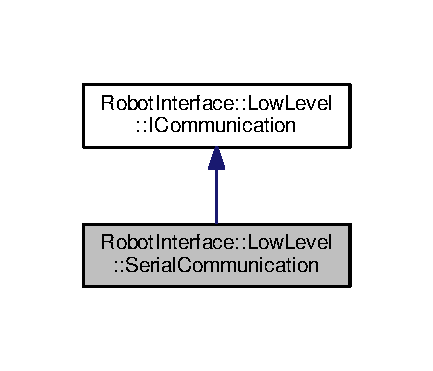
\includegraphics[width=208pt]{classRobotInterface_1_1LowLevel_1_1SerialCommunication__inherit__graph}
\end{center}
\end{figure}


Collaboration diagram for Robot\+Interface\+:\+:Low\+Level\+:\+:Serial\+Communication\+:
\nopagebreak
\begin{figure}[H]
\begin{center}
\leavevmode
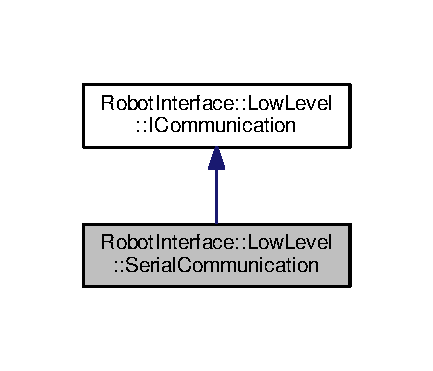
\includegraphics[width=208pt]{classRobotInterface_1_1LowLevel_1_1SerialCommunication__coll__graph}
\end{center}
\end{figure}
\subsection*{Public Member Functions}
\begin{DoxyCompactItemize}
\item 
\hyperlink{classRobotInterface_1_1LowLevel_1_1SerialCommunication_aeb78f679f7b037ca0ecc099fe2cc6e73}{Serial\+Communication} (const std\+::string \&a\+Port)
\begin{DoxyCompactList}\small\item\em initialises a \hyperlink{classRobotInterface_1_1LowLevel_1_1SerialCommunication}{Serial\+Communication} instance \end{DoxyCompactList}\item 
virtual \hyperlink{classRobotInterface_1_1LowLevel_1_1SerialCommunication_a83db7cb65ef662a91f9e7451e85358cb}{$\sim$\+Serial\+Communication} ()\hypertarget{classRobotInterface_1_1LowLevel_1_1SerialCommunication_a83db7cb65ef662a91f9e7451e85358cb}{}\label{classRobotInterface_1_1LowLevel_1_1SerialCommunication_a83db7cb65ef662a91f9e7451e85358cb}

\begin{DoxyCompactList}\small\item\em destructor \end{DoxyCompactList}\item 
bool \hyperlink{classRobotInterface_1_1LowLevel_1_1SerialCommunication_a82fe3bcbc561e158ab7722f7182a97d7}{send\+Command} (const std\+::string \&str)
\begin{DoxyCompactList}\small\item\em validates send goal and sends it to the S\+S\+C32U \end{DoxyCompactList}\end{DoxyCompactItemize}


\subsection{Detailed Description}
deriving from \hyperlink{classRobotInterface_1_1LowLevel_1_1ICommunication}{I\+Communication}\+: class that implement the send command for a serial connection 

\subsection{Constructor \& Destructor Documentation}
\index{Robot\+Interface\+::\+Low\+Level\+::\+Serial\+Communication@{Robot\+Interface\+::\+Low\+Level\+::\+Serial\+Communication}!Serial\+Communication@{Serial\+Communication}}
\index{Serial\+Communication@{Serial\+Communication}!Robot\+Interface\+::\+Low\+Level\+::\+Serial\+Communication@{Robot\+Interface\+::\+Low\+Level\+::\+Serial\+Communication}}
\subsubsection[{\texorpdfstring{Serial\+Communication(const std\+::string \&a\+Port)}{SerialCommunication(const std::string &aPort)}}]{\setlength{\rightskip}{0pt plus 5cm}Robot\+Interface\+::\+Low\+Level\+::\+Serial\+Communication\+::\+Serial\+Communication (
\begin{DoxyParamCaption}
\item[{const std\+::string \&}]{a\+Port}
\end{DoxyParamCaption}
)}\hypertarget{classRobotInterface_1_1LowLevel_1_1SerialCommunication_aeb78f679f7b037ca0ecc099fe2cc6e73}{}\label{classRobotInterface_1_1LowLevel_1_1SerialCommunication_aeb78f679f7b037ca0ecc099fe2cc6e73}


initialises a \hyperlink{classRobotInterface_1_1LowLevel_1_1SerialCommunication}{Serial\+Communication} instance 


\begin{DoxyParams}{Parameters}
{\em a\+Port} & the path to the port which will be used for communication \\
\hline
\end{DoxyParams}


\subsection{Member Function Documentation}
\index{Robot\+Interface\+::\+Low\+Level\+::\+Serial\+Communication@{Robot\+Interface\+::\+Low\+Level\+::\+Serial\+Communication}!send\+Command@{send\+Command}}
\index{send\+Command@{send\+Command}!Robot\+Interface\+::\+Low\+Level\+::\+Serial\+Communication@{Robot\+Interface\+::\+Low\+Level\+::\+Serial\+Communication}}
\subsubsection[{\texorpdfstring{send\+Command(const std\+::string \&str)}{sendCommand(const std::string &str)}}]{\setlength{\rightskip}{0pt plus 5cm}bool Robot\+Interface\+::\+Low\+Level\+::\+Serial\+Communication\+::send\+Command (
\begin{DoxyParamCaption}
\item[{const std\+::string \&}]{str}
\end{DoxyParamCaption}
)\hspace{0.3cm}{\ttfamily [virtual]}}\hypertarget{classRobotInterface_1_1LowLevel_1_1SerialCommunication_a82fe3bcbc561e158ab7722f7182a97d7}{}\label{classRobotInterface_1_1LowLevel_1_1SerialCommunication_a82fe3bcbc561e158ab7722f7182a97d7}


validates send goal and sends it to the S\+S\+C32U 

\begin{DoxyReturn}{Returns}
true if goal is reachable 

false if goal is unreachable 
\end{DoxyReturn}


Implements \hyperlink{classRobotInterface_1_1LowLevel_1_1ICommunication_a88fc73dd43eb0444895e1a8b33fc1623}{Robot\+Interface\+::\+Low\+Level\+::\+I\+Communication}.



The documentation for this class was generated from the following files\+:\begin{DoxyCompactItemize}
\item 
world\+\_\+ws/src/robot\+\_\+interface/src/\+Robot\+Interface/\+Low\+Level/Serial\+Communication.\+hpp\item 
world\+\_\+ws/src/robot\+\_\+interface/src/\+Robot\+Interface/\+Low\+Level/Serial\+Communication.\+cpp\end{DoxyCompactItemize}

\hypertarget{classRobotInterface_1_1HighLevel_1_1Servo}{}\section{Robot\+Interface\+:\+:High\+Level\+:\+:Servo Class Reference}
\label{classRobotInterface_1_1HighLevel_1_1Servo}\index{Robot\+Interface\+::\+High\+Level\+::\+Servo@{Robot\+Interface\+::\+High\+Level\+::\+Servo}}


This class is used for angle calculation and \hyperlink{classRobotInterface_1_1HighLevel_1_1Servo}{Servo} operations.  




{\ttfamily \#include $<$Servo.\+hpp$>$}

\subsection*{Public Member Functions}
\begin{DoxyCompactItemize}
\item 
\hyperlink{classRobotInterface_1_1HighLevel_1_1Servo_a55ee280ff7ceb68f1280689c946db913}{Servo} ()\hypertarget{classRobotInterface_1_1HighLevel_1_1Servo_a55ee280ff7ceb68f1280689c946db913}{}\label{classRobotInterface_1_1HighLevel_1_1Servo_a55ee280ff7ceb68f1280689c946db913}

\begin{DoxyCompactList}\small\item\em explicit edefault constructor \end{DoxyCompactList}\item 
\hyperlink{classRobotInterface_1_1HighLevel_1_1Servo_ae6d458646c8b397b78f259e5c487a422}{Servo} (unsigned long an\+Id, unsigned long a\+Max\+P\+WM, short a\+Max\+Angle, unsigned long a\+Min\+P\+WM, short a\+Min\+Angle)
\begin{DoxyCompactList}\small\item\em initialises a \hyperlink{classRobotInterface_1_1HighLevel_1_1Servo}{Servo} instance \end{DoxyCompactList}\item 
\hyperlink{classRobotInterface_1_1HighLevel_1_1Servo_a8359af04d4e43df4da7d122721abe6e6}{Servo} (const \hyperlink{classRobotInterface_1_1HighLevel_1_1Servo}{Servo} \&rhs)
\begin{DoxyCompactList}\small\item\em copy constructor used for containers \end{DoxyCompactList}\item 
virtual \hyperlink{classRobotInterface_1_1HighLevel_1_1Servo_ac1e9f3039c1b88239124746e4901434d}{$\sim$\+Servo} ()\hypertarget{classRobotInterface_1_1HighLevel_1_1Servo_ac1e9f3039c1b88239124746e4901434d}{}\label{classRobotInterface_1_1HighLevel_1_1Servo_ac1e9f3039c1b88239124746e4901434d}

\begin{DoxyCompactList}\small\item\em destructor of a \hyperlink{classRobotInterface_1_1HighLevel_1_1Servo}{Servo} \end{DoxyCompactList}\item 
unsigned long \hyperlink{classRobotInterface_1_1HighLevel_1_1Servo_a2b2c9e642fe5c546bcff661dc2a3c3be}{convert\+To\+Pwm} (short an\+Angle) const 
\begin{DoxyCompactList}\small\item\em converts an angle to a P\+WM signal \end{DoxyCompactList}\item 
short \hyperlink{classRobotInterface_1_1HighLevel_1_1Servo_aa21ba9d390292c8d89cac23ba0fe0ba4}{convert\+To\+Angle} (unsigned long a\+P\+WM)
\begin{DoxyCompactList}\small\item\em converts a P\+WM signal to an angle \end{DoxyCompactList}\item 
\hyperlink{classRobotInterface_1_1HighLevel_1_1Servo}{Servo} \& \hyperlink{classRobotInterface_1_1HighLevel_1_1Servo_a4d4cc819ba46142c6c3c484748564f4d}{operator=} (const \hyperlink{classRobotInterface_1_1HighLevel_1_1Servo}{Servo} \&rhs)
\begin{DoxyCompactList}\small\item\em assignment operator used for containers \end{DoxyCompactList}\item 
short \hyperlink{classRobotInterface_1_1HighLevel_1_1Servo_a2baa9e28317f6082132558892cb9feef}{get\+Current\+Angle} () const 
\begin{DoxyCompactList}\small\item\em getter that returns the current angle of a \hyperlink{classRobotInterface_1_1HighLevel_1_1Servo}{Servo} \end{DoxyCompactList}\item 
void \hyperlink{classRobotInterface_1_1HighLevel_1_1Servo_a4767afffc5c122d9781444680e9314fe}{set\+Current\+Angle} (short an\+Angle)
\begin{DoxyCompactList}\small\item\em function that sets the current angle of a servo \end{DoxyCompactList}\item 
unsigned long \hyperlink{classRobotInterface_1_1HighLevel_1_1Servo_a4c7c2e4b7538f50e415705221be50aa8}{get\+Id} () const 
\begin{DoxyCompactList}\small\item\em function that gets the ID of a servo \end{DoxyCompactList}\item 
short \hyperlink{classRobotInterface_1_1HighLevel_1_1Servo_ad9324253a759e4169026301539f62a34}{get\+Max\+Angle} () const 
\begin{DoxyCompactList}\small\item\em function that gets the maximum angle a servo is allowed to have \end{DoxyCompactList}\item 
short \hyperlink{classRobotInterface_1_1HighLevel_1_1Servo_a02084d3c842037948cfb8940a9f4a696}{get\+Min\+Angle} () const 
\begin{DoxyCompactList}\small\item\em function that gets the minimum angle a servo is allowed to have \end{DoxyCompactList}\end{DoxyCompactItemize}


\subsection{Detailed Description}
This class is used for angle calculation and \hyperlink{classRobotInterface_1_1HighLevel_1_1Servo}{Servo} operations. 

\subsection{Constructor \& Destructor Documentation}
\index{Robot\+Interface\+::\+High\+Level\+::\+Servo@{Robot\+Interface\+::\+High\+Level\+::\+Servo}!Servo@{Servo}}
\index{Servo@{Servo}!Robot\+Interface\+::\+High\+Level\+::\+Servo@{Robot\+Interface\+::\+High\+Level\+::\+Servo}}
\subsubsection[{\texorpdfstring{Servo(unsigned long an\+Id, unsigned long a\+Max\+P\+W\+M, short a\+Max\+Angle, unsigned long a\+Min\+P\+W\+M, short a\+Min\+Angle)}{Servo(unsigned long anId, unsigned long aMaxPWM, short aMaxAngle, unsigned long aMinPWM, short aMinAngle)}}]{\setlength{\rightskip}{0pt plus 5cm}Robot\+Interface\+::\+High\+Level\+::\+Servo\+::\+Servo (
\begin{DoxyParamCaption}
\item[{unsigned long}]{an\+Id, }
\item[{unsigned long}]{a\+Max\+P\+WM, }
\item[{short}]{a\+Max\+Angle, }
\item[{unsigned long}]{a\+Min\+P\+WM, }
\item[{short}]{a\+Min\+Angle}
\end{DoxyParamCaption}
)}\hypertarget{classRobotInterface_1_1HighLevel_1_1Servo_ae6d458646c8b397b78f259e5c487a422}{}\label{classRobotInterface_1_1HighLevel_1_1Servo_ae6d458646c8b397b78f259e5c487a422}


initialises a \hyperlink{classRobotInterface_1_1HighLevel_1_1Servo}{Servo} instance 


\begin{DoxyParams}{Parameters}
{\em an\+Id} & servo ID \\
\hline
{\em a\+Max\+P\+WM} & the maximum P\+WM signal that the \hyperlink{classRobotInterface_1_1HighLevel_1_1Servo}{Servo} can move to \\
\hline
{\em a\+Max\+Angle} & the maximum angle the \hyperlink{classRobotInterface_1_1HighLevel_1_1Servo}{Servo} can move to \\
\hline
{\em a\+Min\+P\+WM} & the minimum P\+WM signal that the \hyperlink{classRobotInterface_1_1HighLevel_1_1Servo}{Servo} can move to \\
\hline
{\em a\+Min\+Angle} & the minimum angle the \hyperlink{classRobotInterface_1_1HighLevel_1_1Servo}{Servo} can move to \\
\hline
\end{DoxyParams}
\index{Robot\+Interface\+::\+High\+Level\+::\+Servo@{Robot\+Interface\+::\+High\+Level\+::\+Servo}!Servo@{Servo}}
\index{Servo@{Servo}!Robot\+Interface\+::\+High\+Level\+::\+Servo@{Robot\+Interface\+::\+High\+Level\+::\+Servo}}
\subsubsection[{\texorpdfstring{Servo(const Servo \&rhs)}{Servo(const Servo &rhs)}}]{\setlength{\rightskip}{0pt plus 5cm}Robot\+Interface\+::\+High\+Level\+::\+Servo\+::\+Servo (
\begin{DoxyParamCaption}
\item[{const {\bf Servo} \&}]{rhs}
\end{DoxyParamCaption}
)}\hypertarget{classRobotInterface_1_1HighLevel_1_1Servo_a8359af04d4e43df4da7d122721abe6e6}{}\label{classRobotInterface_1_1HighLevel_1_1Servo_a8359af04d4e43df4da7d122721abe6e6}


copy constructor used for containers 


\begin{DoxyParams}{Parameters}
{\em rhs} & the right hand side \hyperlink{classRobotInterface_1_1HighLevel_1_1Servo}{Servo} \\
\hline
\end{DoxyParams}


\subsection{Member Function Documentation}
\index{Robot\+Interface\+::\+High\+Level\+::\+Servo@{Robot\+Interface\+::\+High\+Level\+::\+Servo}!convert\+To\+Angle@{convert\+To\+Angle}}
\index{convert\+To\+Angle@{convert\+To\+Angle}!Robot\+Interface\+::\+High\+Level\+::\+Servo@{Robot\+Interface\+::\+High\+Level\+::\+Servo}}
\subsubsection[{\texorpdfstring{convert\+To\+Angle(unsigned long a\+P\+W\+M)}{convertToAngle(unsigned long aPWM)}}]{\setlength{\rightskip}{0pt plus 5cm}short Robot\+Interface\+::\+High\+Level\+::\+Servo\+::convert\+To\+Angle (
\begin{DoxyParamCaption}
\item[{unsigned long}]{a\+P\+WM}
\end{DoxyParamCaption}
)}\hypertarget{classRobotInterface_1_1HighLevel_1_1Servo_aa21ba9d390292c8d89cac23ba0fe0ba4}{}\label{classRobotInterface_1_1HighLevel_1_1Servo_aa21ba9d390292c8d89cac23ba0fe0ba4}


converts a P\+WM signal to an angle 


\begin{DoxyParams}{Parameters}
{\em a\+P\+WM} & the P\+WM signal to be converted \\
\hline
\end{DoxyParams}
\begin{DoxyReturn}{Returns}
short the angle corresponding to the P\+WM signal 
\end{DoxyReturn}
\index{Robot\+Interface\+::\+High\+Level\+::\+Servo@{Robot\+Interface\+::\+High\+Level\+::\+Servo}!convert\+To\+Pwm@{convert\+To\+Pwm}}
\index{convert\+To\+Pwm@{convert\+To\+Pwm}!Robot\+Interface\+::\+High\+Level\+::\+Servo@{Robot\+Interface\+::\+High\+Level\+::\+Servo}}
\subsubsection[{\texorpdfstring{convert\+To\+Pwm(short an\+Angle) const }{convertToPwm(short anAngle) const }}]{\setlength{\rightskip}{0pt plus 5cm}unsigned long Robot\+Interface\+::\+High\+Level\+::\+Servo\+::convert\+To\+Pwm (
\begin{DoxyParamCaption}
\item[{short}]{an\+Angle}
\end{DoxyParamCaption}
) const}\hypertarget{classRobotInterface_1_1HighLevel_1_1Servo_a2b2c9e642fe5c546bcff661dc2a3c3be}{}\label{classRobotInterface_1_1HighLevel_1_1Servo_a2b2c9e642fe5c546bcff661dc2a3c3be}


converts an angle to a P\+WM signal 


\begin{DoxyParams}{Parameters}
{\em an\+Angle} & the angle to be converted \\
\hline
\end{DoxyParams}
\begin{DoxyReturn}{Returns}
unsigned long the P\+WM signal corresponding to the angle 
\end{DoxyReturn}
\index{Robot\+Interface\+::\+High\+Level\+::\+Servo@{Robot\+Interface\+::\+High\+Level\+::\+Servo}!get\+Current\+Angle@{get\+Current\+Angle}}
\index{get\+Current\+Angle@{get\+Current\+Angle}!Robot\+Interface\+::\+High\+Level\+::\+Servo@{Robot\+Interface\+::\+High\+Level\+::\+Servo}}
\subsubsection[{\texorpdfstring{get\+Current\+Angle() const }{getCurrentAngle() const }}]{\setlength{\rightskip}{0pt plus 5cm}short Robot\+Interface\+::\+High\+Level\+::\+Servo\+::get\+Current\+Angle (
\begin{DoxyParamCaption}
{}
\end{DoxyParamCaption}
) const}\hypertarget{classRobotInterface_1_1HighLevel_1_1Servo_a2baa9e28317f6082132558892cb9feef}{}\label{classRobotInterface_1_1HighLevel_1_1Servo_a2baa9e28317f6082132558892cb9feef}


getter that returns the current angle of a \hyperlink{classRobotInterface_1_1HighLevel_1_1Servo}{Servo} 

\begin{DoxyReturn}{Returns}
short the current angle 
\end{DoxyReturn}
\index{Robot\+Interface\+::\+High\+Level\+::\+Servo@{Robot\+Interface\+::\+High\+Level\+::\+Servo}!get\+Id@{get\+Id}}
\index{get\+Id@{get\+Id}!Robot\+Interface\+::\+High\+Level\+::\+Servo@{Robot\+Interface\+::\+High\+Level\+::\+Servo}}
\subsubsection[{\texorpdfstring{get\+Id() const }{getId() const }}]{\setlength{\rightskip}{0pt plus 5cm}unsigned long Robot\+Interface\+::\+High\+Level\+::\+Servo\+::get\+Id (
\begin{DoxyParamCaption}
{}
\end{DoxyParamCaption}
) const}\hypertarget{classRobotInterface_1_1HighLevel_1_1Servo_a4c7c2e4b7538f50e415705221be50aa8}{}\label{classRobotInterface_1_1HighLevel_1_1Servo_a4c7c2e4b7538f50e415705221be50aa8}


function that gets the ID of a servo 

\begin{DoxyReturn}{Returns}
unsigned long the id to return 
\end{DoxyReturn}
\index{Robot\+Interface\+::\+High\+Level\+::\+Servo@{Robot\+Interface\+::\+High\+Level\+::\+Servo}!get\+Max\+Angle@{get\+Max\+Angle}}
\index{get\+Max\+Angle@{get\+Max\+Angle}!Robot\+Interface\+::\+High\+Level\+::\+Servo@{Robot\+Interface\+::\+High\+Level\+::\+Servo}}
\subsubsection[{\texorpdfstring{get\+Max\+Angle() const }{getMaxAngle() const }}]{\setlength{\rightskip}{0pt plus 5cm}short Robot\+Interface\+::\+High\+Level\+::\+Servo\+::get\+Max\+Angle (
\begin{DoxyParamCaption}
{}
\end{DoxyParamCaption}
) const}\hypertarget{classRobotInterface_1_1HighLevel_1_1Servo_ad9324253a759e4169026301539f62a34}{}\label{classRobotInterface_1_1HighLevel_1_1Servo_ad9324253a759e4169026301539f62a34}


function that gets the maximum angle a servo is allowed to have 

\begin{DoxyReturn}{Returns}
short the maximum angle 
\end{DoxyReturn}
\index{Robot\+Interface\+::\+High\+Level\+::\+Servo@{Robot\+Interface\+::\+High\+Level\+::\+Servo}!get\+Min\+Angle@{get\+Min\+Angle}}
\index{get\+Min\+Angle@{get\+Min\+Angle}!Robot\+Interface\+::\+High\+Level\+::\+Servo@{Robot\+Interface\+::\+High\+Level\+::\+Servo}}
\subsubsection[{\texorpdfstring{get\+Min\+Angle() const }{getMinAngle() const }}]{\setlength{\rightskip}{0pt plus 5cm}short Robot\+Interface\+::\+High\+Level\+::\+Servo\+::get\+Min\+Angle (
\begin{DoxyParamCaption}
{}
\end{DoxyParamCaption}
) const}\hypertarget{classRobotInterface_1_1HighLevel_1_1Servo_a02084d3c842037948cfb8940a9f4a696}{}\label{classRobotInterface_1_1HighLevel_1_1Servo_a02084d3c842037948cfb8940a9f4a696}


function that gets the minimum angle a servo is allowed to have 

\begin{DoxyReturn}{Returns}
short the minimum angle 
\end{DoxyReturn}
\index{Robot\+Interface\+::\+High\+Level\+::\+Servo@{Robot\+Interface\+::\+High\+Level\+::\+Servo}!operator=@{operator=}}
\index{operator=@{operator=}!Robot\+Interface\+::\+High\+Level\+::\+Servo@{Robot\+Interface\+::\+High\+Level\+::\+Servo}}
\subsubsection[{\texorpdfstring{operator=(const Servo \&rhs)}{operator=(const Servo &rhs)}}]{\setlength{\rightskip}{0pt plus 5cm}{\bf Servo} \& Robot\+Interface\+::\+High\+Level\+::\+Servo\+::operator= (
\begin{DoxyParamCaption}
\item[{const {\bf Servo} \&}]{rhs}
\end{DoxyParamCaption}
)}\hypertarget{classRobotInterface_1_1HighLevel_1_1Servo_a4d4cc819ba46142c6c3c484748564f4d}{}\label{classRobotInterface_1_1HighLevel_1_1Servo_a4d4cc819ba46142c6c3c484748564f4d}


assignment operator used for containers 


\begin{DoxyParams}{Parameters}
{\em rhs} & the right hand side \hyperlink{classRobotInterface_1_1HighLevel_1_1Servo}{Servo} \\
\hline
\end{DoxyParams}
\begin{DoxyReturn}{Returns}
\hyperlink{classRobotInterface_1_1HighLevel_1_1Servo}{Servo}\& the newly assigned servo 
\end{DoxyReturn}
\index{Robot\+Interface\+::\+High\+Level\+::\+Servo@{Robot\+Interface\+::\+High\+Level\+::\+Servo}!set\+Current\+Angle@{set\+Current\+Angle}}
\index{set\+Current\+Angle@{set\+Current\+Angle}!Robot\+Interface\+::\+High\+Level\+::\+Servo@{Robot\+Interface\+::\+High\+Level\+::\+Servo}}
\subsubsection[{\texorpdfstring{set\+Current\+Angle(short an\+Angle)}{setCurrentAngle(short anAngle)}}]{\setlength{\rightskip}{0pt plus 5cm}void Robot\+Interface\+::\+High\+Level\+::\+Servo\+::set\+Current\+Angle (
\begin{DoxyParamCaption}
\item[{short}]{an\+Angle}
\end{DoxyParamCaption}
)}\hypertarget{classRobotInterface_1_1HighLevel_1_1Servo_a4767afffc5c122d9781444680e9314fe}{}\label{classRobotInterface_1_1HighLevel_1_1Servo_a4767afffc5c122d9781444680e9314fe}


function that sets the current angle of a servo 


\begin{DoxyParams}{Parameters}
{\em an\+Angle} & the angle to be set \\
\hline
\end{DoxyParams}


The documentation for this class was generated from the following files\+:\begin{DoxyCompactItemize}
\item 
world\+\_\+ws/src/robot\+\_\+interface/src/\+Robot\+Interface/\+High\+Level/Servo.\+hpp\item 
world\+\_\+ws/src/robot\+\_\+interface/src/\+Robot\+Interface/\+High\+Level/Servo.\+cpp\end{DoxyCompactItemize}

%--- End generated contents ---

% Index
\backmatter
\newpage
\phantomsection
\clearemptydoublepage
\addcontentsline{toc}{chapter}{Index}
\printindex

\end{document}
